% !TEX encoding = UTF-8 Unicode
% program VLNA -- prida ~ tam kde je potřeba je soucasti texlive baliku

\pdfoutput=1
\documentclass[twoside,12pt]{article}
% \usepackage[utf8]{inputenc} 
\usepackage[utf8x]{inputenc}
\usepackage[czech]{babel}
\usepackage{dipp}
\usepackage{listings}
\usepackage{pgfplots, pgfplotstable}
\usepackage{filecontents}
\usepackage{comment}
\usepackage{listings}
\usepackage[export]{adjustbox}
\usepackage{float}
\usepackage[justification=centering]{caption}
\usepackage{colortbl}
\usepackage{tabularx}
\usepackage{mathtools}

\sloppy

\usepackage{array}
\newcolumntype{L}[1]{>{\raggedright\let\newline\\\arraybackslash\hspace{0pt}}m{#1}}
\newcolumntype{C}[1]{>{\centering\let\newline\\\arraybackslash\hspace{0pt}}m{#1}}
\newcolumntype{R}[1]{>{\raggedleft\let\newline\\\arraybackslash\hspace{0pt}}m{#1}}

\clubpenalty 10000
\widowpenalty 10000

%
%
% START
\begin{document}

\def\,{\penalty10000\hskip.25em}
\pagestyle{headings}
\cislovat{2}

\bakalarska


\titul{Hra založená na rozšířené realitě pro platformu iOS}{Aleš Kocur}{Ing. David Procházka, Ph.D.}{Brno~2015}


\podekovani{
Chtěl bych především poděkovat svým rodičům za jejich důslednou podporu v průběhu celého studia, přítelkyni za shovívavost nad mými hodinami strávenými před počítačem, kolegům z The Funtasty za brainstorming při vymýšlení konceptu a také Ing. Davidu Procházkovi, Ph.D. za příkladné vedení práce a cenné připomínky, rady a nápady.
}

\prohlasenimuz{V~Brně dne \today}
 
\newpage\null\thispagestyle{empty}\newpage

\abstrakt{
Tato práce se zabývá rozšířenou realitou a jejím využitím ve hrách na~platformě iOS. Zkoumá aktuální přístupy her, které rozšířenou realitu využívají. Práce popisuje jejich koncepty interakce a přidaných hodnot oproti běžným hrám (bez rozšířené reality). Dále jsou představeny frameworky umožňující implementaci aplikací založených na rozšířené realitě pro mobilní platformu iOS a jejich srovnání na základě vhodnosti pro tvorbu hry. Poslední částí práce je návrh vlastní hry s důrazem na vyřešení či zamezení nedostatků vypozorovaných na již existujících hrách a jejich konceptech a následná implementace s použitím nejlépe ohodnoceného frameworku.
}{}

\abstract{
The paper discusses an augmented reality and its integration in games for iOS platform. It considers different kinds of approaches used in currently popular augmented reality games, namely their concepts and their benefits over usual games (without usage of the augmented reality). It describes frameworks that can be used to develop applications with an augmented reality for iOS and comparison of their features and suitability to be the foundation of an augmented reality game. The final section describes designing my own game which aims to avoid critical drawbacks found by observing existing games.
}{}

\klicovaslova{rozšířená realita, iOS, objective-c, Metaio knihovna}{}

\keywords{augmented reality, iOS, objective-c, Metaio framework}{}

\obsah

%
% úvod a cíl práce
%
\kapitola{Úvod a cíl práce}

% 
\sekce{Úvod}
Myšlenku rozšířené reality (angl. \textit{Augmented reality}) nastínil již před více než sto lety americký spisovatel \textit{Lyman Frank Baum} \cite{baum}, ale až v posledních letech s nástupem mobilních technologií získává na svém potencionálu více než kdy předtím. Mobilní technologie a přenositelná zařízení nám umožňují pomocí senzorů snímat naše okolí a obohacovat ji o uměle vytvořené prvky. Toho se dá využít v celé škále odvětví jako je zábavní průmysl, medicína, marketing, vzdělávání, navigace, sport a mnoho dalšího. Mobilní zařízení jsou v současné době nejrychleji rostoucím odvětvím \cite{mobile_economy}, jejich hardwarové konfigurace zajišťují prostředky pro bezproblémové vykreslování detailních modelů i chod herního enginu. Mnohé firmy vidí v AR a VR (Virtual reality) budoucnost hraní a proto investují do jejich výzkumu \cite{guardian_samsung}. Tato práce se zabývá aplikací rozšířené reality v zábavním průmyslu, konkrétně hrami. 

% 
% Cíl práce
\sekce{Cíl práce}
Cílem práce je prozkoumat možnosti her v rozšířené realitě na mobilní plaformě iOS a vytvořit hru, která bude rozšířené reality využívat jako obohacujícího prvku pro hráče. Prvním a zároveň velmi důležitým krokem je zvolení správného frameworku na základě výše uvedených kritérií. Poté je potřeba důkladně navrhnout herní systém a využití rozšířené reality. Dalším krokem bude připravení grafických podkladů a modelů pro hru a následně samotná implementaci. Poslední kapitoly jsou pak věnovány uživatelskému testování, vyhodnocení a úvahami nad možnými vylepšeními.

%
% Rozšířená realita
%

\kapitola{Rozšířená realita}
Rozšířenou realitou (angl. \textit{Augmented reality}) je označováno zobrazování digitálních objektů (3D modelů, 2D obrazů) v reálném světě. Tohoto efektu lze dosáhnout pomocí tzv. okna, které nám sdružuje reálné prostředí s virtuálním. Může se jednat o jakoukoliv formu displaye od mobilního telefonu, až po sofistikované nástroje, jako jsou speciální brýle (např. \textit{Google Glass}). Digitálním objektům je možné pomocí různých technik analýzy obrazu specifikovat pozici, natočení a velikost. Metody vizuálního sledování lze rozdělit do třech základních kategorií \cite{klein_visual_tracking}.

\sekce{Metody vizuálního sledování}
\podsekce{Marker tracking}
Jedním z nejjednodušších a také nejspolehlivějších rozpoznávacích technik postavení objektů je \textit{Marker Tracking}. Jedná se většinou o černobíle čtvercové \textit{QR kódy}, které uchovávají informaci o svém identifikačním čísle, orámované černým okrajem o pevné velikosti. Na základě přečteného identifikátoru lze přiřazovat jednotlivým markerům různé objekty. Černé rámování slouží k analýze vzdálenosti od markeru, jeho natočení a velikost. Tato metoda je velmi efektivní, analýza takového markeru na zařízení \textit{iPhone 5} s frameworkem \textit{Metaio} v obrazu zabere průměrně 4,3 ms (na základě vlastního měření). Další výhodou této metody je možnost definice velkého množství markerů s různým identifikátorem a na každém identifikátoru pak lze zobrazovat odlišné objekty.

\begin{figure}[H]
    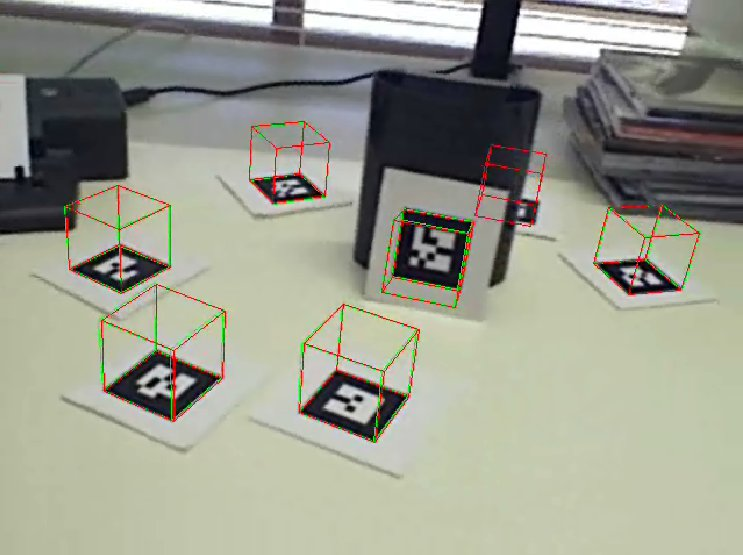
\includegraphics[width=330px, center]{images/marker-tracking.jpg}
    \caption{VTTResearch, \textit{Marker tracking}.
	[online]. [cit.~2015-04-02]. Obrázek ve formátu: JPEG. Dostupné z: http://virtual.vtt.fi/virtual/proj2/multimedia/media/images/MultiMarker.jpg}
    \label{marker_tracking}
\end{figure}

\podsekce{Markerless tracking}
Další možností jak umisťovat objekty do rozšířené reality je pomocí tzv. \textit{Markerless trackingu}. Jedná se o princip podobný Marker trackingu s tím rozdílem, že namísto markerů jsou použity libovolné obrazy. Při analýze je pak potřeba vlastnit digitální předlohu takového obrazu a vyhledávat jej ve snímané realitě. Na základě porovnání natočení obrazu ve snímané realitě a předlohy je zjištěna aktuální vzdálenost od objektu, velikost a natočení. Z důvodu zrychlení je v průběhu snímání porovnáván vzor z posledního sejmutého frame. Tento princip analýzy může být pomalejší zvláště při špatných světelných podmínkách \cite{handbook_of_ar}.

\begin{figure}[H]
    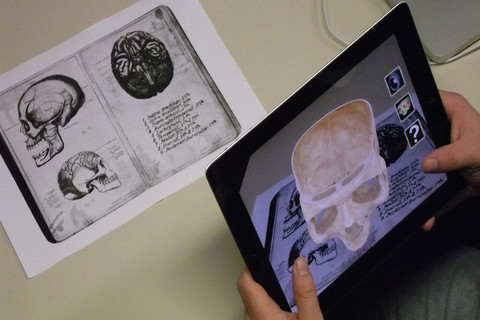
\includegraphics[width=350px, center]{images/markerless-tracking.jpg}
    \caption{Wikipedia, \textit{Markerless tracking}. [online]. [cit. 2015-04-02].
	Obrázek ve formátu: JPEG. Dostupné z: http://upload.wikimedia.org/wikipedia/commons/f/f4/App\_iSkull,\_an\_augmented \_human\_skull.jpg}
    \label{markerless_tracking}
\end{figure}

\podsekce{Sledování neznámých prostředí}
Umisťovat virtuální objekty do snímané reality lze i bez známých vzorů a to pomocí detekce hran na základě pohybu kamery. Nejrozšířenější systémy takovéto analýzy jsou \textit{SLAM (Simultaneous localization and mapping)} a jeho vylepšení \textit{PTAM (Parallel Tracking and Mapping)}. \textit{PTAM} je vyvíjen \textit{Active Vision Laboratory na University of Oxford} a od roku 2014 volně dostupný pod licencí \textit{GNU GPLv3}. Tento systém dokáže analyzovat plochy a hrany v obrazu a na základě těchto informací pak vykreslovat správně umístěné a natočené virtuální objekty. Tyto systémy mají uplatnění mimo jiné také při navigaci autopilotovaného vozidla, vesmírných vozů a podobně.

\begin{figure}[H]
    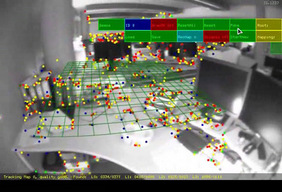
\includegraphics[width=350px, center]{images/slam.jpg}
    
    \caption{Department of Engineering Science, University of Oxford, \textit{SLAM: Simultaneous localization and mapping}
	[online]. [cit. 2015-04-02]. 
	Obrázek ve formátu: JPEG. Dostupné z: http://www.robots.ox.ac.uk/~lav/Papers/castle\_etal\_iswc2008/castle\_etal\_iswc2008.jpg}
    \label{slam}
\end{figure}

\sekce{Srovnání}
Z uvedených informací vyplývá, že implementačně nejjednodušším a nejdostupnějším řešením je Marker tracking za předpokladu potřeby rozpoznání více konkrétních míst v realitě. Mírně složitější, ale zato uživatelsky přívětivější řešení nabízí Markerless tracking v podobě možnosti rozpoznávání vzorů a obrázků. Pro situace, kdy nepotřebujeme nacházet konkrétní pozice, ale spíše plochy, je zde řešení typu SLAM, které je však z uvedených typů nejnáročnější na implementaci.

%
% Aktuální hry a jejich koncepty
%

\kapitola{Využití rozšířené reality, koncepty využité ve hrách}
Rozšířená realita nabývá s vývojem stále výkonější mobilních telefonů na atraktivitě a rozšiřuje se i v komerční svéře. Mobilní aplikace dokáží interagovat s realitou např. přehráváním trailerů k filmům nad jeho plakátem, vizualizovat návrhy staveb nad prospekty nebo vizualizovat učební materiál v interaktivních učebnicích. Využití rozšířené reality je nespočetné a s přibývající dostupností technologií roste i počet nápadů na její uplatnění. Velké oblibě se těší zejména ve hrách, kde využívá prostředí hráče jako herní plochu a mobilní telefon jako okno do rozšířené reality.

\sekce{Interakce se zařízením}
Tento koncept je postaven na principu interakce hráče pouze se zařízením. Hráč vůbec nemanipuluje ani neinteraguje s prvky herního pole. Tento koncept je vhodný pro zejména pro typy her ve kterých nepotřebujeme pohybovat s objekty a je charakteristický pro mapově (geolokačně) založené hry -- objekty jsou umisťovány do reálného světa s koodináty. Typickým představitelem takového konceptu je hra \textit{Ingress}.

%
% Ingress
% 

\podsekce{Ingress}
Masově multiplayerová online hra vyvíjená startupem \textit{Niantics Labs}, kterou zaštiťuje \textit{Google}, dostupná pro \textit{iOS} i \textit{Android}. Celá hra má v pozadí příběh o \uv{Exotické hmotě} (\textit{Exotic Matter}), která byla objevena vědci z \textit{CERNu}, a je to zárodek mimozemského druhu zvaného Shapers. Osvícení (The Enlightened), jedna ze dvou frakcí, věří, že toto je úsvit nového věku. Druhá frakce, Rezistence (The Resistance) naopak brojí proti těmto mimozemským silám. Hra spočívá ve vytváření frakčních portálů na různých místech, zejména na městských památkách, veřejných budovách a podobně. Hráči chodí s telefony po městě a vytvářením takovýchto portálů přivlastňují danná uzemí své frakci. Mohou také stavět obranné prvky a bránit tak tyto portály před napadením frakce druhé. Zobrazování rozšířené reality je zjednodušené, pouze černé pozadí s obrysy některých budov. Hra se tedy více než na rozšířenou realitu zaměřuje na příběh a rozšířená realita zde slouží pouze jako část celé hry. Více informací lze získat na oficiálních webových stránkách hry \textit{www.ingress.com} \cite{ingress}.


\begin{figure}[H]
    \centering
    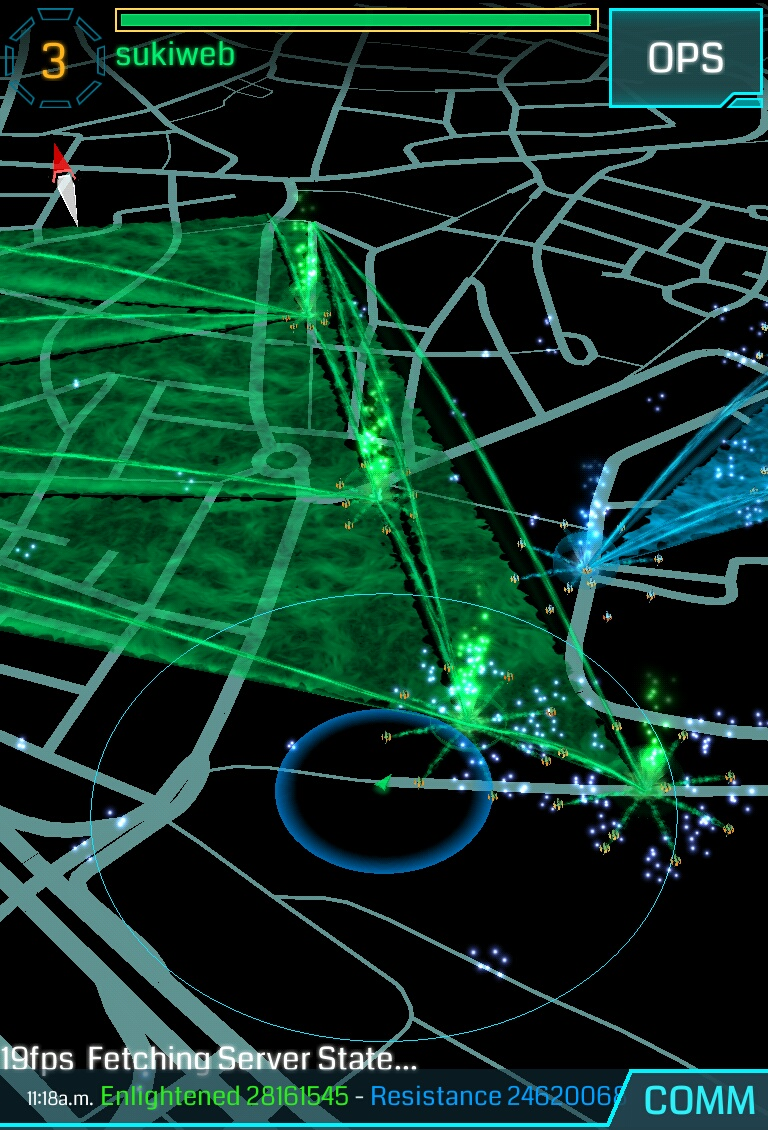
\includegraphics[width=320px, center]{images/ingress.jpg}
    \caption{\textit{Screenshot ze hry Ingress}. Yahoo Inc. Flickr [online]. [cit. 2015-04-02]. Obrázek ve formátu: JPEG. Dostupné z: https://farm9.staticflickr.com/8219/8266348091\_08fe415355\_o.jpg}
    \label{ingress_screenshot}
\end{figure}

\sekce{Interakce s herní deskou}
Dalším konceptem je interakce s herní deskou, kdy hráč interaguje pomocí gest nebo stisknutím virtuálních tlačítek na desce. Tento koncept štěpí interakční část a zobrazovací (hráč manipuluje s prvky na desce, ale výsledek vidí pouze přes zařízení) a pro uživatele může být v případech mobilního telefonu obzvlášť nepříjemný na ovládání, více vhodný je například na brýle. Z tohoto důvodu je také tento koncept v mobilních hrách téměř nepoužívaný. Mezi hry využívající tohoto přístupu jsou povětšinou hry původem deskové či karetní a rozšířenou realitu zde využívají spíše pro zvýšení intenzity zážitku ze hry vizualizacema procesů, které si jinak člověk musí pouze představovat. 

%
% Drakerz-Confrontation 
%

\podsekce{Drakerz Confrontation}
Karetní hra vyvíjená od roku 2010 francouzskou firmou \textit{Peoleo} s první alpha verzí vydanou roku 2013 ve Francii \cite{venturebeat}. Dnes je hra dostupná pouze pro PC a nejsou žádné informace, zda dorazí v budoucnu i na mobilní platformy. \textit{Drakerz Confrontation} hráči mají karty s různými typy draků s různými vlastnostmi a schopnostmi. Hra využívá rozšířené reality k vizualizaci draků nad kartami položenými na stole. Ke hraní je potřeba vlastnit kameru připojitelnou k PC, na kterém se pak vizualizace zobrazují. Vizualizované jsou jak pohyby draků po herní ploše, tak např. boje i prostoje. Více informací lze nalézt na oficiálních stránkách hry \textit{www.drakerz.com} \cite{peoleo_about}, kde je také možné zakoupit karty nebo hru stáhnout.


\begin{figure}[H]
    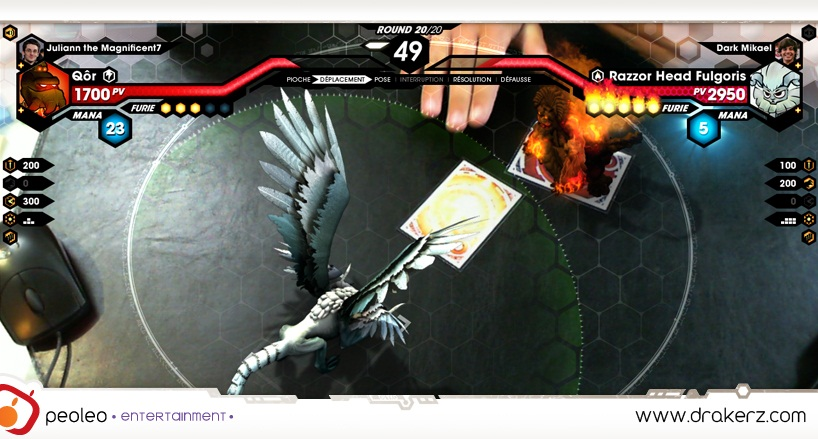
\includegraphics[width=424px, center]{images/drakerz-confrontation.jpg}
    \caption{\textit{Screenshot ze hry Drakerz Confrontation}. Game guide
	[online]. [cit.~2015-04-02]. Obrázek ve formátu: JPEG. Dostupné z: http://game-guide.fr/wp-content/uploads/2014/03/drakerz-confrontation-05.jpg}
    \label{drakerz_screenshot}
\end{figure}

\sekce{Smíšená interakce}
Tento koncept kombinuje předchozí dva uvedené. Hráč v tomto případě primárně používá zařízení, ale má i možnost ovládat herní prvky v reálném prostřední na herní desce. Typickým příkladem smíšené interakce je hra \textit{ARHrrrr!}.

% 
% ARHrrrr!
\podsekce{ARHrrrr!}
Jednou z populárních her je hra \textit{ARhrrrr!} z dílny \textit{Georgia Tech Augmented Environments Lab}, která využívá vytištěné hrací plochy k vizualizaci části města (\textit{Markerless tracking}), kterou napadají zombie a hráč v roli snipera v helikoptéře se pohybuje nad hrací plochou a střílí. Tento koncept s herní plochou a ovládáním výhradně přes zařízení je doplněn o ruzné podpůrné fukce ovládáné pomocí interakce se snímaným prostředím. Jako příklad lze uvést, že položením bonbónu \textit{Skittles} na herní plochu vznikne nášlapná mina, kterou můžeme kliknutím na ni odjistit (příklad interakce s herní plochou). Různé barvy bonbónů mají navíc různé funkce.

\begin{figure}[H]
    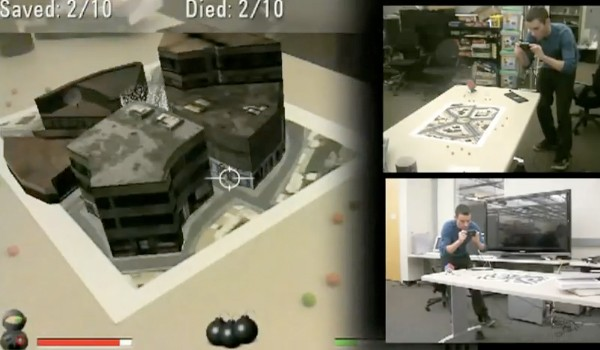
\includegraphics[width=424px, center]{images/arhrrrr.jpg}
    \caption{\textit{Screenshot ze hry ARhrrrr!}.
	[online]. [cit.~2015-04-02]. Obrázek ve~formátu: JPEG. Dostupné z: http://www.blogcdn.com/www.engadget.com/media/2009/06/arhrrrr-pic-rm-eng.jpg
}
    \label{arhrrrr_screenshot}
\end{figure}

\sekce{Shrnutí}
Hry využívají rozdílných konceptů podle úlohy, kterou rozšířená realita ve hře zastává. Hra \textit{Ingress} nám příkladně ukazuje využití konceptu interakce se zařízením, není zde potřeba nijak ovlivňovat hru prostřednictvím reality. Na takovém principu staví povětšinou karetní a deskové hry, jako příklad zde uvedena hra \textit{Drakerz Confrontation}. Tento přístup není moc uplatnitelný na mobilních zařízeních, je zde výhodnější použít statickou kameru. Třetím konceptem je pak kombinace dvou výše zmíněných, který nám dovoluje ovládat hru jak přes zařízení, tak přes realitu. Výhody tohoto konceptu jsou popsány na hře \textit{ARHrrrr!}.

% 
% Nova stranka
\newpage 

\kapitola{Framework}

\sekce{Kritéria hodnocení}
Kritéria hodnocení se odvíjí od náročnosti požadavků na aplikaci, v tomto případě hra. Je tedy důležité, aby framework uměl dobře pracovat s 3D modely a provádět animace, aby hra byla zajímavá. Dalším aspektem je rychlost závislá na počtu zobrazovaných objektů a posledním neméně důležitým faktorem jsou licenční podmínky pro používání.

\sekce{Přehled frameworků}

\podsekce{ARToolKit}
\textit{ARToolkit} byl původně vyvinut \textit{Hirokazu Katou na Nara Institute of Science and Technology} v roce 1999. Nyní je udržován \textit{The Human Interface Technology Lab na University of Washington} jako open source projekt s komerčníma licencema od \textit{ARToolWork}.

\begin{figure}[H]
    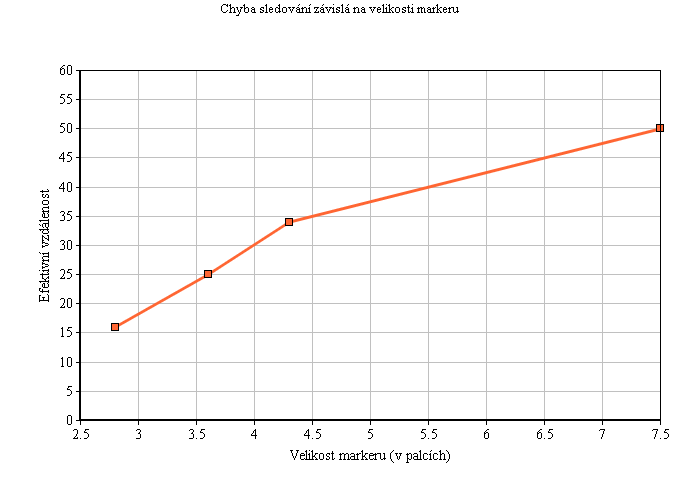
\includegraphics[width=400px, center]{images/artoolkit_benchmark.png}
    \caption{Chyba sledování závislá na velikosti markeru, Podle originálu: \textit{The Human Interface Technology Lab, University of Washington ARToolKit Benchmarks}
	[online]. [cit. 2015-04-03]. Dostupné z: http://www.hitl.washington.edu/artoolkit/documentation/benchmark.htm
}
    \label{artoolkit_benchmark}
\end{figure}
 Tento framework je dostupný pro všechny majoritní platformy (\textit{Windows, Linux, OS X, SGI}) s různými porty pro mobilní operační systémy (\textit{iOS, Android}). Mobilní verze tohoto frameworku portují již konkrétní firmy a vydávají jako vlastní produkt, nejsou tedy volně dostupné -- nepodařilo se sestavit testovací projekt pro tento framework a benchmarky uvedené v dokumentaci jsou velmi nepřesně specifikované (chybí specifikace hardwaru, na kterém byly tyto měření prováděny). 

Mezi hlavní fukce frameworku patří kamerově pozicované a orientováné sledování, sledování černých čtverců s možností definice vlastních typů, jednoduchá kalibrace kamer \cite{artoolkit_features}. Podpora vykreslování modelů je pouze nízkoúrovňová, lze renderovat objekty pomocí \textit{OpenGL}. Většinou je využit v projektech jako část komplexního toolkitu pro práci s rozšířenou realitou např. \textit{OSGART} (kombinace \textit{ARToolKit} a \textit{OpenSceneGraph}) \cite{osgart} nebo \textit{ARToolKitPlus} (rozšířená verze \textit{ARToolKitu}, vývoj ukončen roku 2006) \cite{wagner_schmalstieg}. 

\podsekce{Metaio}
\textit{Metaio} je multiplatformní framework který vyvíjí stejnojmenná německá firma od roku 2003. Mezi produkty \textit{Metaio} najdeme framework pro rozšířenou realitu na všechny majoritní platformy a také sadu aplikačních nástrojů specializující se na usnadnění práce i samotný vývoj bez programování. \textit{Metaio} pro \textit{iOS} je dostupné jako \textit{C++} framework. 
Dokumentace uvádí měření, ukazující udržení výkonu vykreslování 60 snímků za vteřinu (FPS) při 200 000 polygonech na \textit{iPhone 5S}.

\begin{figure}[H]
\centering
    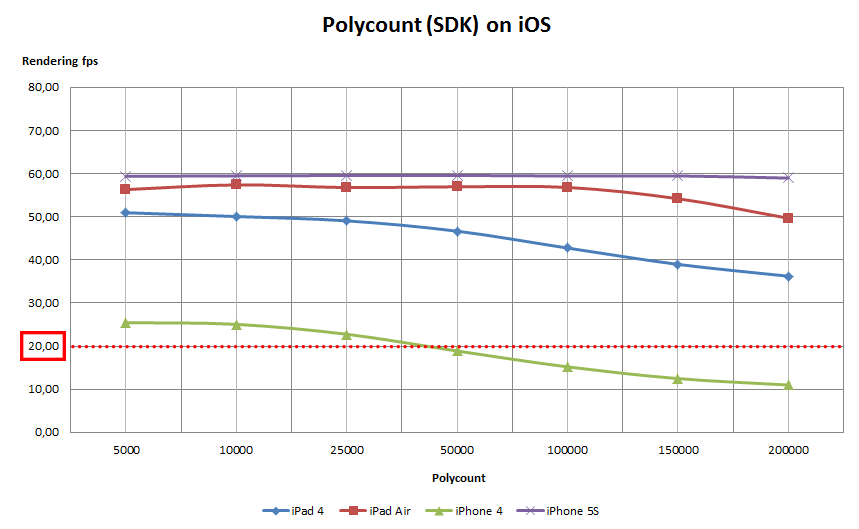
\includegraphics[width=424px, center]{images/Polycount_SDK_iOS_20fps.png}
\captionsetup{justification=centering}
    \caption{Metaio GmbH, \textit{Rychlost vykreslování (v FPS) pro jednotlivé iOS zařízení závislé na počtu vykreslovaných polygonů}.
	[online]. [cit. 2015-04-03]. 
	Dostupné z: http://dev.metaio.com/sdk/documentation/content-creation/3d-animation/polygon-count/general-guidelines/}
    \label{metaio_benchmark}
\end{figure}

Také byl vytvořen testovací projekt, jehož jediný múkolem bylo rozeznávat 20~různých markerů. Na tomto projektu pak byly provedeny zkoušky rychlosti nalezení markeru v obrazu. Test byl prováděn na zařízení \textit{iPhone 5} (model A1429) firmy \textit{Apple}. Z výsledných hodnot byl vypočítán průměr 4,31 ms. 


\textit{Metaio SDK} dokáže pracovat s modely ve formátech \textit{OBJ}, \textit{MD2} a \textit{FBX} a podporuje také jejich animace. Pod podmínkou vodoznaku a nemožnosti publikovat aplikaci na \textit{AppStore} nabízí volnou licenci na všechny verze svého frameworku. 

\podsekce{Qualcomm Vuforia}
Jedná se o poměrně nový framework vyvíjený od roku 2011 a nabízí velké množství funkcí. Jako hlavní lze uvést tzv. markerless recognition (možnost vykreslovat objekty nad obrázky), podporu frameworku \textit{Unity} (framework usnadňující vývoj 3D her) nebo takzvané virtuální tlačítka (\textit{Virtual buttons}, tlačítka promítaná do virtuální reality a interakce s nimi). Samotný framework nabízí aplikační rozhraní pro \textit{C++}, \textit{Javu}, \textit{Objective-C} a \textit{.NET}, což významným způsobem usnadňuje portace aplikace na různé platformy. Široké spektrum funkcí se odráží na licenčních podmínkách frameworku, u neplacených licencí je omezen počet rozpoznaných objektů (pozn. v průběhu tvorby této práce byly změněny licenční podmínky a framework je dostupný zdarma s vodoznakem a nemožností publikovat aplikaci). Velkým mínusem je stejně jako v případě \textit{ARToolKitu} pouze nízkoúrovňová podpora vykreslování objektů pomocí \textit{OpenGL}. Pro podporu zobrazování modelů ve formátech např. \textit{OBJ}, \textit{FBX} a podobně je potřeba využít nějaké další pomocné knihovny \cite{vuforia_3dformats}.

\podsekce{Augmented kit}
Framework psaný čistě pro platformu \textit{iOS} a tedy v \textit{Objective-C}. Vyniká jednoduchým API a dobrou dokumentací. Nabízí pouze základní služby vykreslovaní objektů na markerech, či GPS souřadnic a gyroskopu. Framework je vyvíjen teprve od roku 2012 firmou \textit{Luteg Software Technologies} a to se projevuje velmi malou vývojářskou základnou. Na druhou stranu má přívětivé licenční podmínky, kdy poskytuje volnou licenci pod podmínkou vodoznaku a nemožnosti aplikaci publikovat na \textit{AppStore}. 

\newpage
\kapitola{Metodika}
Pro zvolení správných technologií je nutné jako první navrhnout konceptuální model celé hry. Na základě tohoto modelu je pak potřeba zvolit technologie tak, abychom dosáhli danných kritérií. Konkrétně se jedná o volbu frameworku, 3D formátu pro modely a modelovací nástroj.

\sekce{Koncept hry}
Nosným prvkem celé hry je rozšířená realita. Na základě informací o možných typech trackingu jsem zvolil jako trackingovou metodu marker tracking pro její jednoduchou implementaci a možnost rozlišení markerů podle identifikátorů. Základem hry tedy je pole markerů s různými uspořádáními -- hráč si může zvolit na jakém typu herní plochy chce hrát. Na tomto poli budou vizualizovány herní modely s možností jejich animací. Pro interakci s objekty rozšířené reality je využito konceptu \textit{Interakce se zařízením}. Hra je simulací stavby a řízení vlastního města a je spustitelná na zařízeních se systémem \textit{iOS 8} s primárním cílením pro zařízení \textit{iPad}. 

\sekce{Výběr frameworku}
Pro výběr frameworku byly na základě herního konceptu stanoveny tyto kritéria:
\begin{itemize}
	\item Spustitelnost pod iOS
	\item Marker tracking
	\item Podpora 3D formátu modelů
	\item Animovatelnost modelů
	\item Volná licence / akademická licence
	\item Dokumentace, tutoriály
\end{itemize}

Výsledky pro tyto kritéria jednotlivých představených frameworků můžeme vidět v Tabulce \ref{table:frameworks-compare}.

% Please add the following required packages to your document preamble:
% \usepackage[table,xcdraw]{xcolor}
% If you use beamer only pass "xcolor=table" option, i.e. \documentclass[xcolor=table]{beamer}

\begin{table}[H]
\centering
\resizebox{\textwidth}{!}{%
\begin{tabular}{|
>{\columncolor[HTML]{656565}}l |C{25mm}|
>{\columncolor[HTML]{EFEFEF}}C{25mm} |C{25mm}|C{25mm}|}
\hline
\color[HTML]{FFFFFF}\textbf{Framework}            & \cellcolor[HTML]{C0C0C0}{\color[HTML]{000000} \textbf{ARToolKit}} & \cellcolor[HTML]{C0C0C0}{\color[HTML]{000000} \textbf{Metaio}} & \cellcolor[HTML]{C0C0C0}{\color[HTML]{000000} \textbf{Qualcomm Vuforia}} & \cellcolor[HTML]{C0C0C0}{\color[HTML]{000000} \textbf{Augmented kit}} \\ \hline
\color[HTML]{FFFFFF}Podpora iOS                   & \textit{Částečně}                                                 & \textit{Ano}                                                   & \textit{Ano}                                                             & \textit{Ano}                                                          \\ \hline
\color[HTML]{FFFFFF}Marker tracking       & \cellcolor[HTML]{FFFFFF}\textit{Ano}                              & \textit{Ano}                                                   & \cellcolor[HTML]{FFFFFF}\textit{Ano}                                     & \cellcolor[HTML]{FFFFFF}\textit{Ne}                                   \\ \hline
\color[HTML]{FFFFFF}3D formát modelů      & \textit{Ne, pouze OpenGL}                                         & \textit{OBJ, FBX, MD2}                                         & \textit{Ne, pouze OpenGL}                                                & \textit{Ne}                                                           \\ \hline
\color[HTML]{FFFFFF}Animace               & \textit{Pouze GLUT}                                               & \textit{Ano (FBX, MD2)}                                        & \textit{Pouze GLUT}                                                              & \textit{Ne}                                                           \\ \hline
\color[HTML]{FFFFFF}Licence               & \textit{Komerční}                                                 & \textit{Omezená s vodoznakem}                                  & \textit{Omezená s vodoznakem}                                            & \textit{Omezená s vodoznakem}                                         \\ \hline
\color[HTML]{FFFFFF}Dokumentace/tutoriály & \textit{Ano/ne}                                                   & \textit{Ano/ano}                                               & \textit{Ano/ano}                                                         & \textit{Ano/pouze ukázka}                                             \\ \hline
\end{tabular}
}
\caption{Porovnání frameworků}
\label{table:frameworks-compare}
\end{table}

Po porovnání výsledků byl vyhodnocen jako nejvhodnější framework Metaio, který jako jediný splňuje všechna daná kritéria.

\sekce{Formát 3D modelů}
Základem dobrého návrhu aplikace je správná volba technologií. Mezi ně v tomto případě patří i volba formátu pro 3D modely. Framework Metaio podporuje renderování objektů ve formátech \textit{OBJ}, \textit{MD2} a \textit{FBX}. 
%Pro tvorbu modelů byl použit 3D modelovací nástroj \textit{3Ds Max} od firmy \textit{Autodesk} a to čistě z důvodů základní znalosti tohoto softwaru. Tato práce se nezabývá porovnáváním modelovacích softwarů.
Kritérii pro výběr formátu jsou podpora exportu z \textit{3Ds Max}, podpora animací, podpora textur.

\podsekce{OBJ}
Otevřený formát vyvinutý firmou \textit{Wavefront Technologies} pro přenos 3D objektů. Formát specifikuje pozice každého vertexu v objektu, UV souřadnice textury vertexu a plochy (faces) každého polygonu \cite{obj_wiki}. Obsahuje podporu textur pomocí přiložených materiálů ve formátu \textit{MTL (Material Template Library)}. Formát \textit{OBJ} je standardně textový formát, může se však vyskytovat i v binární podobě. Takovýto binární soubor má pak příponu .mod. Formát bohužel nemá podporu animací \cite{obj_doc} a tím nevyhovuje v jednom ze tří bodů daných kritérií.

\podsekce{MD2}
Formát \textit{MD2} se stal populárním díky firmě \textit{id Software's} \cite{md2_wiki}, která jej použila v \textit{id Tech 2} známý jako \textit{Quake II engine} \cite{quake_engine} pro modely všech postav ve hře \textit{Quake II} a dalších, rovněž postavených na tomto enginu. \textit{MD2} má podporu key-frame animací a textur. \textit{MD2} byl později nahrazen novějším formátem \textit{MD3} \cite{id_tech_3_wiki}. Tento formát je nyní již zastaralý a nemá valnou podporu v \textit{3Ds Maxu}, vyjma komerčního pluginu \cite{qtip_plugin}. 

\podsekce{FBX}
Proprietární formát \textit{FBX} (FilmBoX) je od roku 2006 vyvíjen a spravován firmou \textit{Autodesk} \cite{autodesk_fbx}. Firma pro užívání tohoto formátu vydala \textit{FBX SDK}, který umožňuje zapis, čtení a konverze tohoto formátu \cite{autodesk_fbx_sdk}. Formát podporuje animace, textury a jelikož je vyvíjen stejnou firmou jako \textit{3Ds Max}, má v tomto softwaru i náležitou podporu pro export.

\sekce{Shrnutí}

\begin{table}[H]
\begin{tabular}{|c|c|c|c|}
\hline
\rowcolor[HTML]{656565} 
{\color[HTML]{FFFFFF} Formát}                      & {\color[HTML]{FFFFFF} Podpora animací} & {\color[HTML]{FFFFFF} Podpora textur} & {\color[HTML]{FFFFFF} Podpora exportu 3Ds Max}  \\ \hline
\rowcolor[HTML]{FFFFFF} 
\cellcolor[HTML]{C0C0C0}{\color[HTML]{000000} OBJ} & Ne                                     & Ano                                   & Ano                                             \\ \hline
\rowcolor[HTML]{FFFFFF} 
\cellcolor[HTML]{C0C0C0}{\color[HTML]{000000} MD2} & {\color[HTML]{000000} Ano}             & {\color[HTML]{000000} Ano}            & {\color[HTML]{000000} Pouze komerčním pluginem} \\ \hline
\rowcolor[HTML]{EFEFEF} 
\cellcolor[HTML]{C0C0C0}{\color[HTML]{000000} FBX} & {\color[HTML]{000000} Ano}             & {\color[HTML]{000000} Ano}            & {\color[HTML]{000000} Ano}                      \\ \hline
\end{tabular}
\caption{Porovnání formátů pro reprezentaci 3D modelů}
\label{table:model-format-compare}
\end{table}

Na základě daných kritérií byl zvolen za nejvhodnější formát \textit{FBX}. Metaio sice podporuje tento formát, ale využívá k tomu utility zvané MeshConvertor, které je potřeba dodat \textit{FBX} model s případnými UV mapami textur modelu. Výsledným souborem je archiv formátu \textit{ZIP}, který obsahuje informace o daném modelu, přiložené textury, názvy animací a metadata. Tento \textit{ZIP} pak již lze snadno používat v \textit{Metaio SDK}.

\sekce{Modelovací nástroj}
Jediné kritérium stanovené pro výběr modelovacího nástroje je podpora exportu do \textit{FBX}. Jelikož tuto možnost mají všechny majoritní modelovací nástroje (\textit{Autodesk 3Ds Max}, \textit{Blender}, \textit{Maya}, \dots), rozhodl jsem se pro použití \textit{3Ds Maxu} od firmy \textit{Autodesk} pouze na základě předešlých znalostí prostředí tohoto programu. \textit{Autodesk} poskytuje na své produkty akademickou licenci.


% 
% Nova stranka
\newpage

\kapitola{ARCity}

\sekce{Rozbor konceptu}
Základní koncept hry spočívá v budování města -- budov -- a řízení ekonomiky tohoto města -- od toho znikl název ARCity -- ovlivňováním ekonomických parametrů (DPH, počet volných pracovních míst, obyvatelné parcely). Hra se je vizualizována na hrací desce. Rozměr hrací desky lze měnit přidáním další desky a tím navýšit rozměry z 5$\times$5 na 5$\times$10 až 5$\times$15 markerů. Větší rozměry nejsou podporovány a to zejména z důvodů hardwarové náročnosti. Každý marker představuje parcelu pro vytvoření takzvané zóny. Základní surovinou pro řízení hry jsou peníze. Základními ukazateli jsou pak spokojenost a počet obyvatel.  Za peníze může hráč nechat na prázných parcelách vystavět specifické zóny. Základní typy zón jsou čtyři -- obytná zóna, průmyslová zóna, obchodní zóna a kulturní zóna. Každá z těchto zón může ovlivňovat ukazatele, přinášet suroviny (peníze) nebo naopak spotřebovávat. Uprostřed města je již od počátku hry postavena radnice, která slouží k možnosti za určitých podmínek postoupit do vyšší úrovně. Vyšší úroveň nám pak otevírá nové možnosti jak vylepšovat zóny. Cílem hry je postavit město na nejvyšší úrovni. 

Na začátku hry je hráči dovoleno stavět pouze základní zóny bez možnosti je vylepšit. Hráč může takovéto vylepšení odemknout získáním vyšší městské úrovně. Pro získání úrovně je potřeba splnit limity danné pro každou úrověň zvlášť, jedná se o kombinaci počtu obyvatel, jejich spokojenosti a městského rozpočtu. Po splnění těchto požadavků je hráči umožněno vylepšovat své zóny a tím dosáhnout větších profitů, obyvatel, pracovních míst a podobně.

\podsekce{Obytná zóna}
Slouží k navýšení maximálního počtu obyvatel, které může město ubytovat. Počet obyvatel, kteří ve městě žijí (přistěhují se nebo se odstěhují), je závislý na stavu spokojenosti a počtu pracovních míst. Zvýšením úrovně této zóny lze navýšit její obytnou kapacitu až na trojnásobek té základní.

\podsekce{Průmyslová zóna}
Zaměstnává lidi ve městě -- vytváří pracovní místa a generuje peníze. Snižuje však kulturu města (ukazatel spokojenosti). Obdobně lze také zvyšovat nabídku pracovních pozic navýšením úrovně zóny a to až na trojnásobek.

\podsekce{Kulturní zóna}
Zvyšuje spokojenost obyvatel města, ale musí být dotována z městského rozpočtu. Zvýšením úrovně získáme možnost uspokojení více obyvatel za mírně zvýšenou dotaci.

\podsekce{Obchodní zóna}
Stejně jako průmyslová zóna vytváří pracovní místa, ale pouze v menším množství. Nemá však takový vliv na snižování spokojenosti obyvatel. Také generuje malé množství peněz a jedná se o nejdražší zónu. Zvýšením úrovně této zóny zvyšujeme také její přijmy a počet volných pracovních míst. 

\podsekce{Městská správa, radnice}
Základní zóna, kterou má hráč již postavenou na startu hry a nelze ji zničit. Poskytuje možnost řízení velikosti daně a tím ovlivňovat příjmy a spokojenost obyvatel

\sekce{Metaio}
\textit{Metaio SDK} je knihovna napsaná v jazyce \textit{C++} a pro použití v \textit{Cocoa touch} projektu, který je vyvíjen v jazyce \textit{Objective-C} (nebo také nově ve \textit{Swiftu}), stačí knihovnu přilinkovat do tzv. bundle. Pro použití knihoven psaných v \textit{C++} má \textit{Cocoa touch} speciální formát s příponou .mm, kterému se říká \textit{Objective-C++}. Touto příponou dáváme překladači najevo kombinování těchto dvou jazyků v jednom souboru. 

\sekce{Cocoapods}
Pro usnadnění připojování pomocných frameworků do projektu vznikl open source projekt s názvem \textit{Cocoapods}. Tento tzv. dependency manager napsaný v jazyce \textit{Ruby} má za úkol přidávat, odebírat nebo aktualizovat použité externí frameworky. Seznam frameworků je definován textovým sobourem s názvem Podfile, jsou v něm definice zdrojů, verzí a targetu projektu, do kterých mají být frameworky přilinkovány. Veškeré frameworky použité v této hře jsou vydány pod svobodými licencemi (většinou \textit{MIT}).

\podsekce{MagicalRecord}
\textit{MagicalRecord} je framework, který usnadňuje práci s klasickým \textit{Core Data} frameworkem. Zjednodušuje práci s daty zaváděním \textit{Active record} přístupu známého zejména z \textit{Ruby on Rails}. Konkrétně se jedná o udržování defaultních kontextů a jejich vytváření, vytváření, update, mazání objektů a také jejich import. Tento framework je dostupný pod \textit{MIT} licencí \cite{magical_record}.

\podsekce{TFTableDescriptor}
\textit{TFTableDescriptor} slouží jako pomocník při sestavování tabulek. Tabulky lze sestavit pomocí popisu  speciálními třídami \textit{TFTableDescriptor}, \textit{TFSectionDescriptor} a \textit{TFRowDescriptor}. Tento framework je vyvíjen firmou \textit{The Funtasty} pod otevřenou licencí \textit{MIT} \cite{tftabledescriptor}.

\sekce{Model}
Pro vývoj aplikací na platformu \textit{iOS} se využívá takzvaného \textit{MVC} (Model-View-Controller) přístupu. Základní model hry se skládá z těchto tříd:

\begin{itemize}
	\item \textbf{Engine} - jádro hry, řídí celou herní logiku, obsluhuje ostatní komponenty modelu
	\item \textbf{GraphicsCore} - grafické jádro hry, zajišťuje vykreslování objektů na správných markerech, deleguje změny stavů, spouští animace a překládá koordináty
	\item \textbf{GraphicsItem} - představuje jeden vykreslovaný objekt v herní scéně, jejich vytváření je řízeno z CraphicsCore.
	\item \textbf{MetaioSDK} - třída frameworku Metaio, instance této třídy je držena v GraphicsCore a je pomocí ní řízeno vykreslování objektů ve scéně
	\item \textbf{GameSession} - uchovává informace o stavu hry, obsahuje reference na hráče a či herní plochu
	\item \textbf{User} - obsahuje informace o uživateli (peníze, spokojenost, \dots)
	\item \textbf{Plot} - představuje herní parcelu, obsahuje informace o zóně a metody pro jejich vytváření a mazání
	\item \textbf{Zone} - jsou vytvářeny Ploty, obsahují informace na základě typu
\end{itemize}

Jak v modelu jednotlivé třídy figurují je navrženo jednoduchým UML diagramem tříd.

\begin{figure}[H]
\centering
    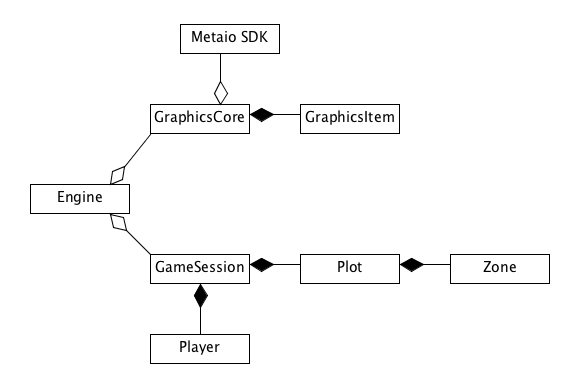
\includegraphics[width=420px, center]{images/model.png}
\captionsetup{justification=centering}
    \caption{Aleš Kocur, \textit{Diagram tříd datového modelu}}
    \label{class_diagram}
\end{figure}

Tento návrh zajišťuje striktní oddělení herní logiky od grafického vykreslování. Pro uchování stavu hry stačí ukládat instance \textit{GameSession} se svými kompozicemi. Uloženou \textit{GameSession} lze pak přiřadit \textit{Enginu}, který dokáže na jejím základě obnovit grafický obraz hry. Grafické jádro monitoruje změny v \textit{GameSession} přiřazené v \textit{Enginu} a na jejich základě provádí změny viditelné části hry. 

\sekce{Uživatelské rozhraní}

Rozhraní, jakým uživatelé, hráči, interagují s prvky hry, jsou kritickou částí návrhu. Důležitou roli zde hrají zaběhlé principy daného systému, řekněme konvence, na které jsou uživatelé zvyklí -- setkávají se s nimy napříč všemi aplikacemi. V případě operačního systému iOS je jednou z hlavních domén uživatelského rozhraní navigační bar umístěný vždy nahoře po celé šířce displaye.    

\begin{figure}[H]
\centering
    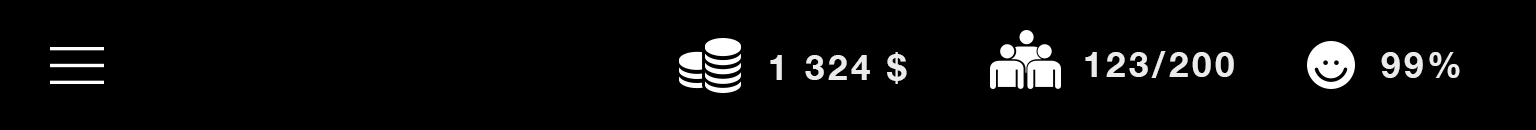
\includegraphics[width=420px, center]{images/nav_bar_iphone.png}
\captionsetup{justification=centering}
    \caption{Aleš Kocur, \textit{Navigation bar ze hry ARCity}}
    \label{navigation_bar}
\end{figure}

Z toho můžeme usoudit, že uživatel je zvyklý veškeré důležité navigační prvky a statická data (např. titulek) hledat právě na tomto místě, a koncipovat návrh tak, abychom všechny statické data a navigační prvky směřovali na horní část obrazovky. Jelikož je vetšinou takovýchto navigačních informací velké množství a zobrazovat jej na každé obrazovce není z hlediska šetření místa pro samotný obsah příliš dobré, začalo se používat, a dnes je již konvencí, menu reprezentované ikonou se třemi vodorovnými čarami (známé také jako \textit{hamburger menu}). 

\begin{figure}[H]
\centering
    
\includegraphics[width=100px, center]{images/hamburger_menu.png}
\captionsetup{justification=centering}
    \caption{Aleš Kocur, \textit{Hamburger menu ze hry ARCity}}
    \label{hamburger-menu}
\end{figure}


Dalším důležitým aspektem návrhu rozhraní je rozměr samotného zařízení. Tato hra je primárně cílena na \textit{iPad}. Máme tedy k dispozici plochu čítající 2048$\times$1536 pixelů s úhlopříčkou 12,9 palce. Hlavním obsahem hry je okno pro zobrazování rozšířené reality, je tudíž nutné pro něj vymezit dostatečně velký prostor. Z daného rozlišení můžeme usoudit, že při natočení zařízení do tzv. \textit{portrait} módu, tj. kratší stranou k sobě, výška displaye představuje oněch 2048 pixelů. Při využití části zhruba 500 pixelů na navigaci a ovládání, získáme přibližně čtvercovou plochu pro zobrazení okna rozšířené reality. Při takovém držení \textit{iPadu} oběma rukama zároveň, využívá hráč k ovládání své palce. Dosah a příjemnost takového ovládání ilustruje \textit{Obrázek 12}.

\begin{figure}[H]
\centering
    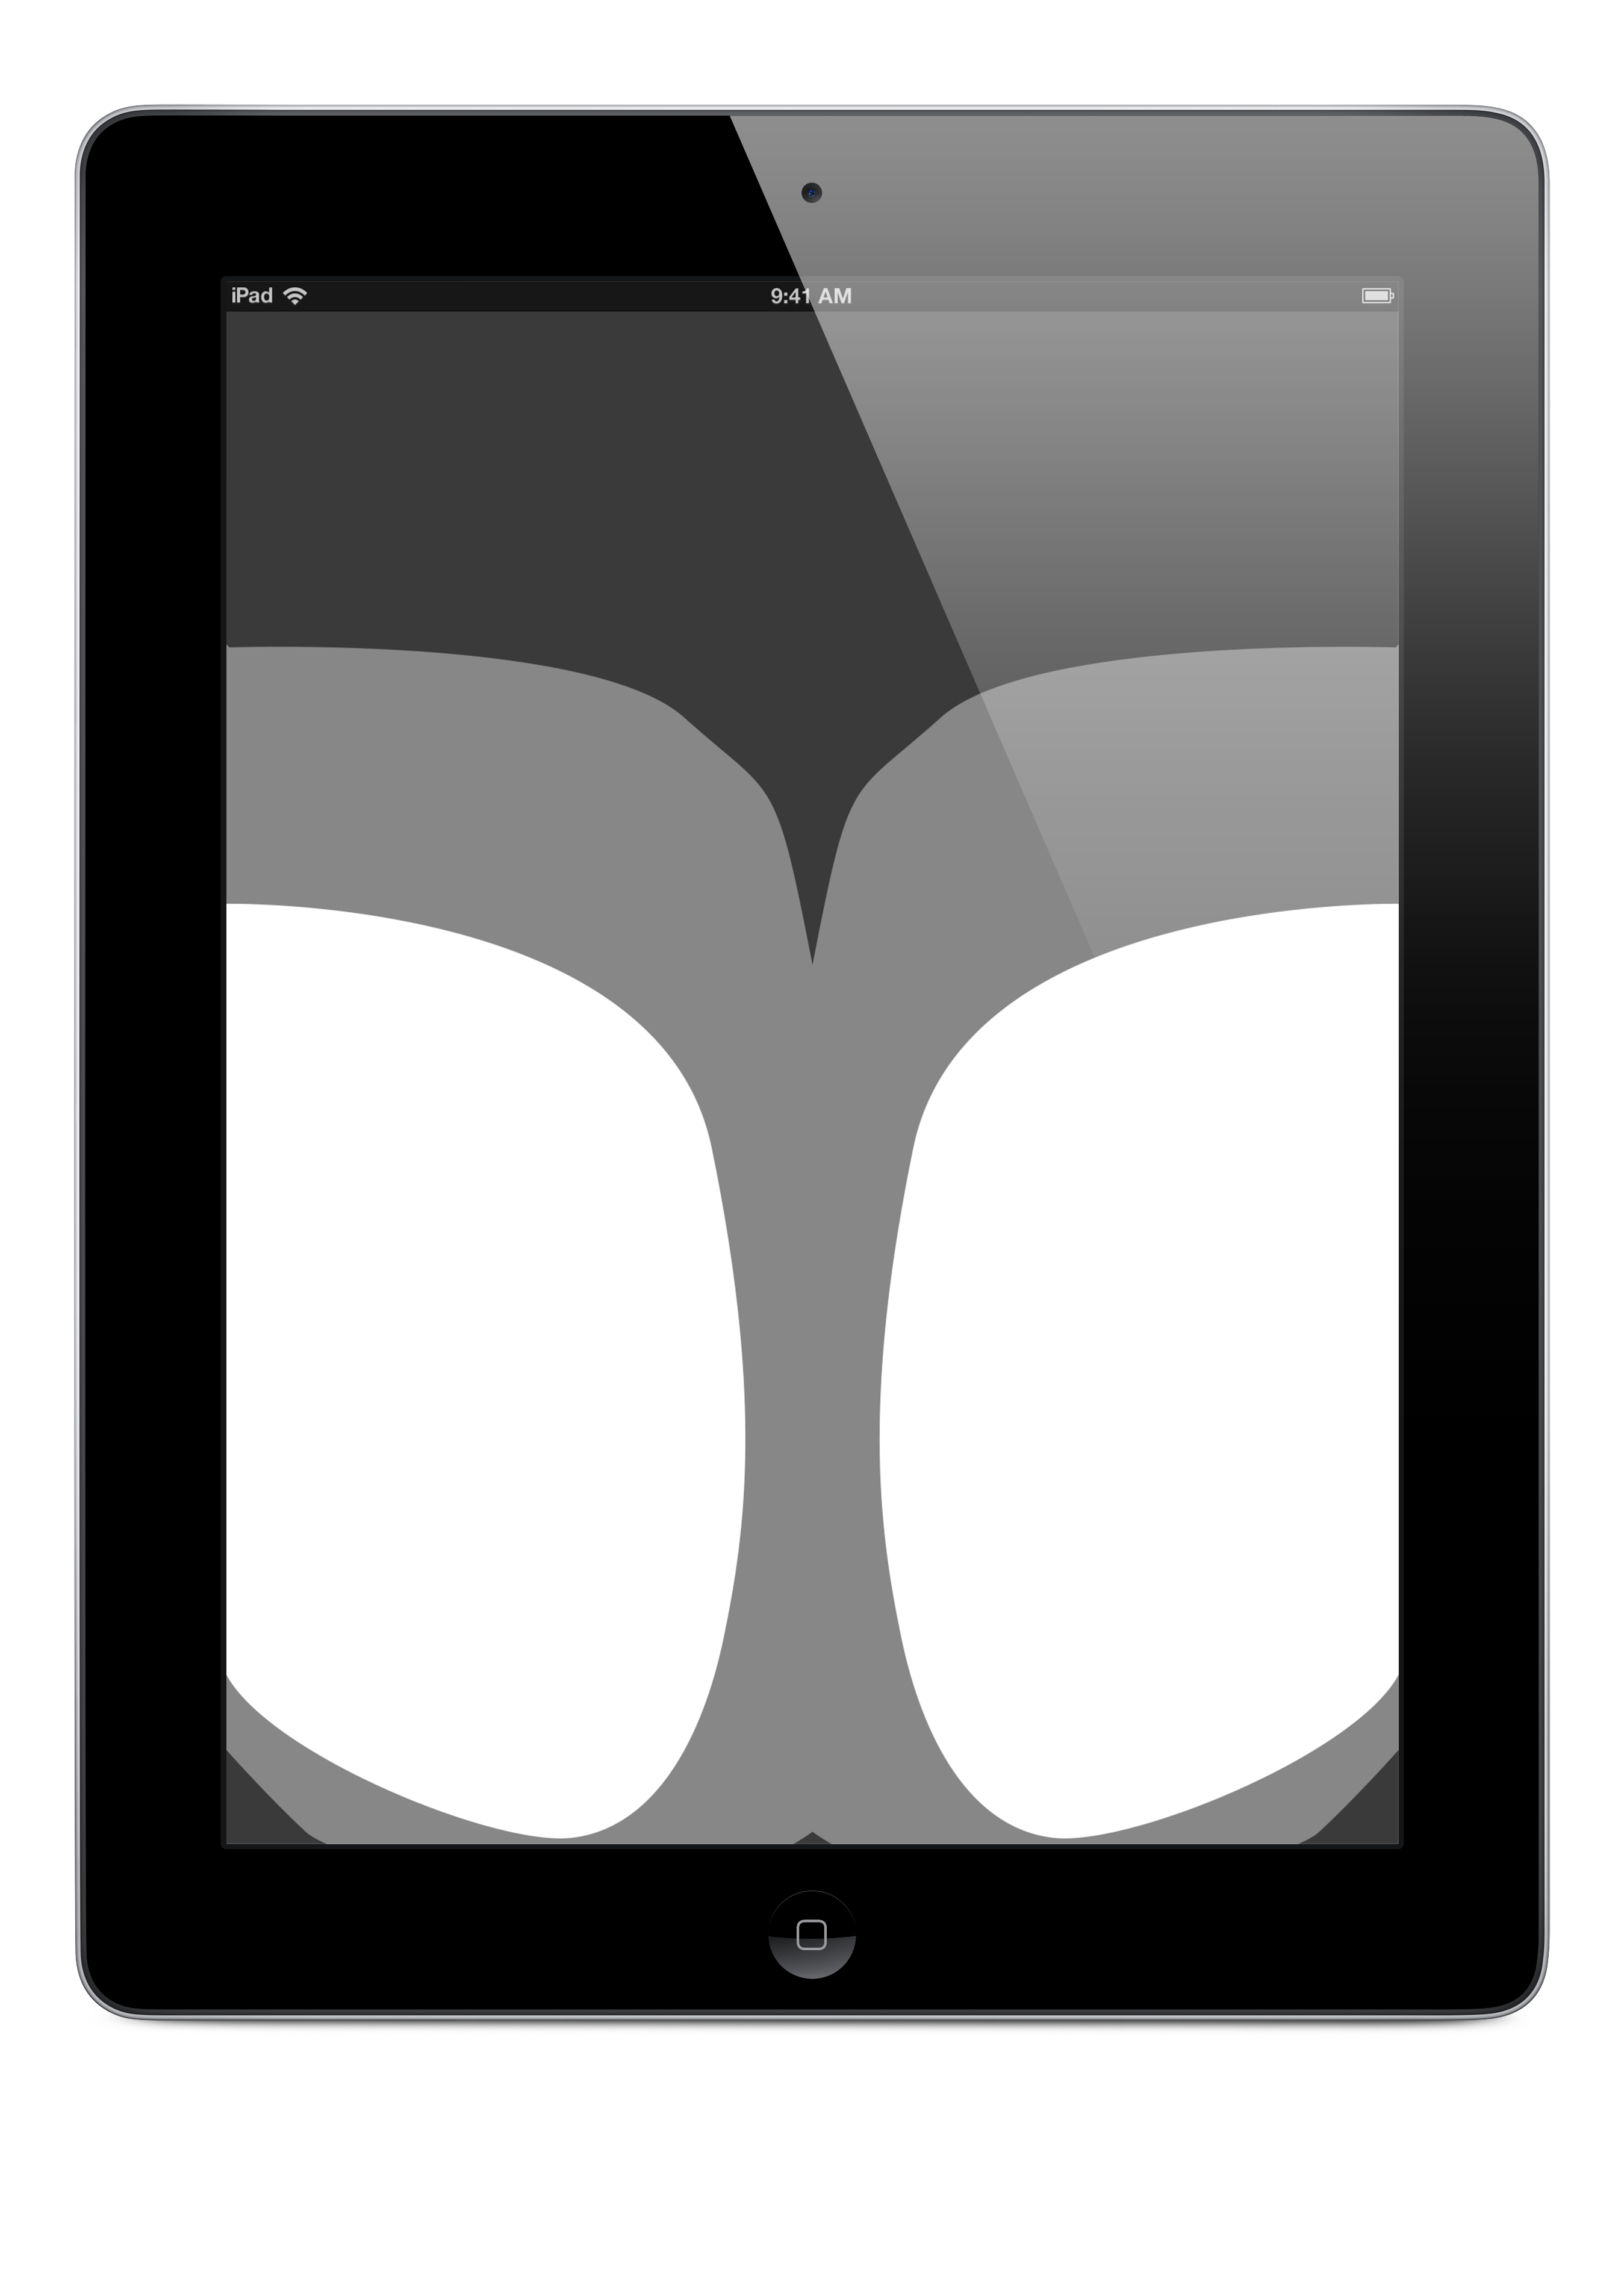
\includegraphics[width=300px, center]{images/ipad-toucharea.png}
\captionsetup{justification=centering}
    \caption{Aleš Kocur, \textit{Rozdělení dosazitelnosti prvků na iPadu 3. generace v portrait módu}, na základě vlastního měření}
    \label{class_diagram}
\end{figure}


Jak můžeme vidět, nejdosažitelnější části displaye se nachází ve spodních části displaye. Na základě takovéto úvahy dojdeme k závěru, že pro snadno dosažitelné ovládací prvky by se mělo ovládání hry vyskytovat někde ve spodní části displaye. Jelikož prostřední část máme vyhrazenou pro okno do rozšířené reality, jediné místo zbývá na spodním okraji displaye. 

Složením výše uvedených věcí do jednoho získáme ideální návrh rozhraní. Horní část o přibližné velikosti 100 pixelů vyčleníme pro navigaci a ukazatele, prostřední část, asi 1500 pixelů pro okno do rozšířené reality a zbylých zhruba 400 px ve spodní části vymezíme na ovládání. Po návrhu konkrétních ovládacích prvků pak můžeme návrh optimalizovat ve prospěch ještě většího okna pro rozšířenou realitu.

\begin{figure}[H]
\centering
    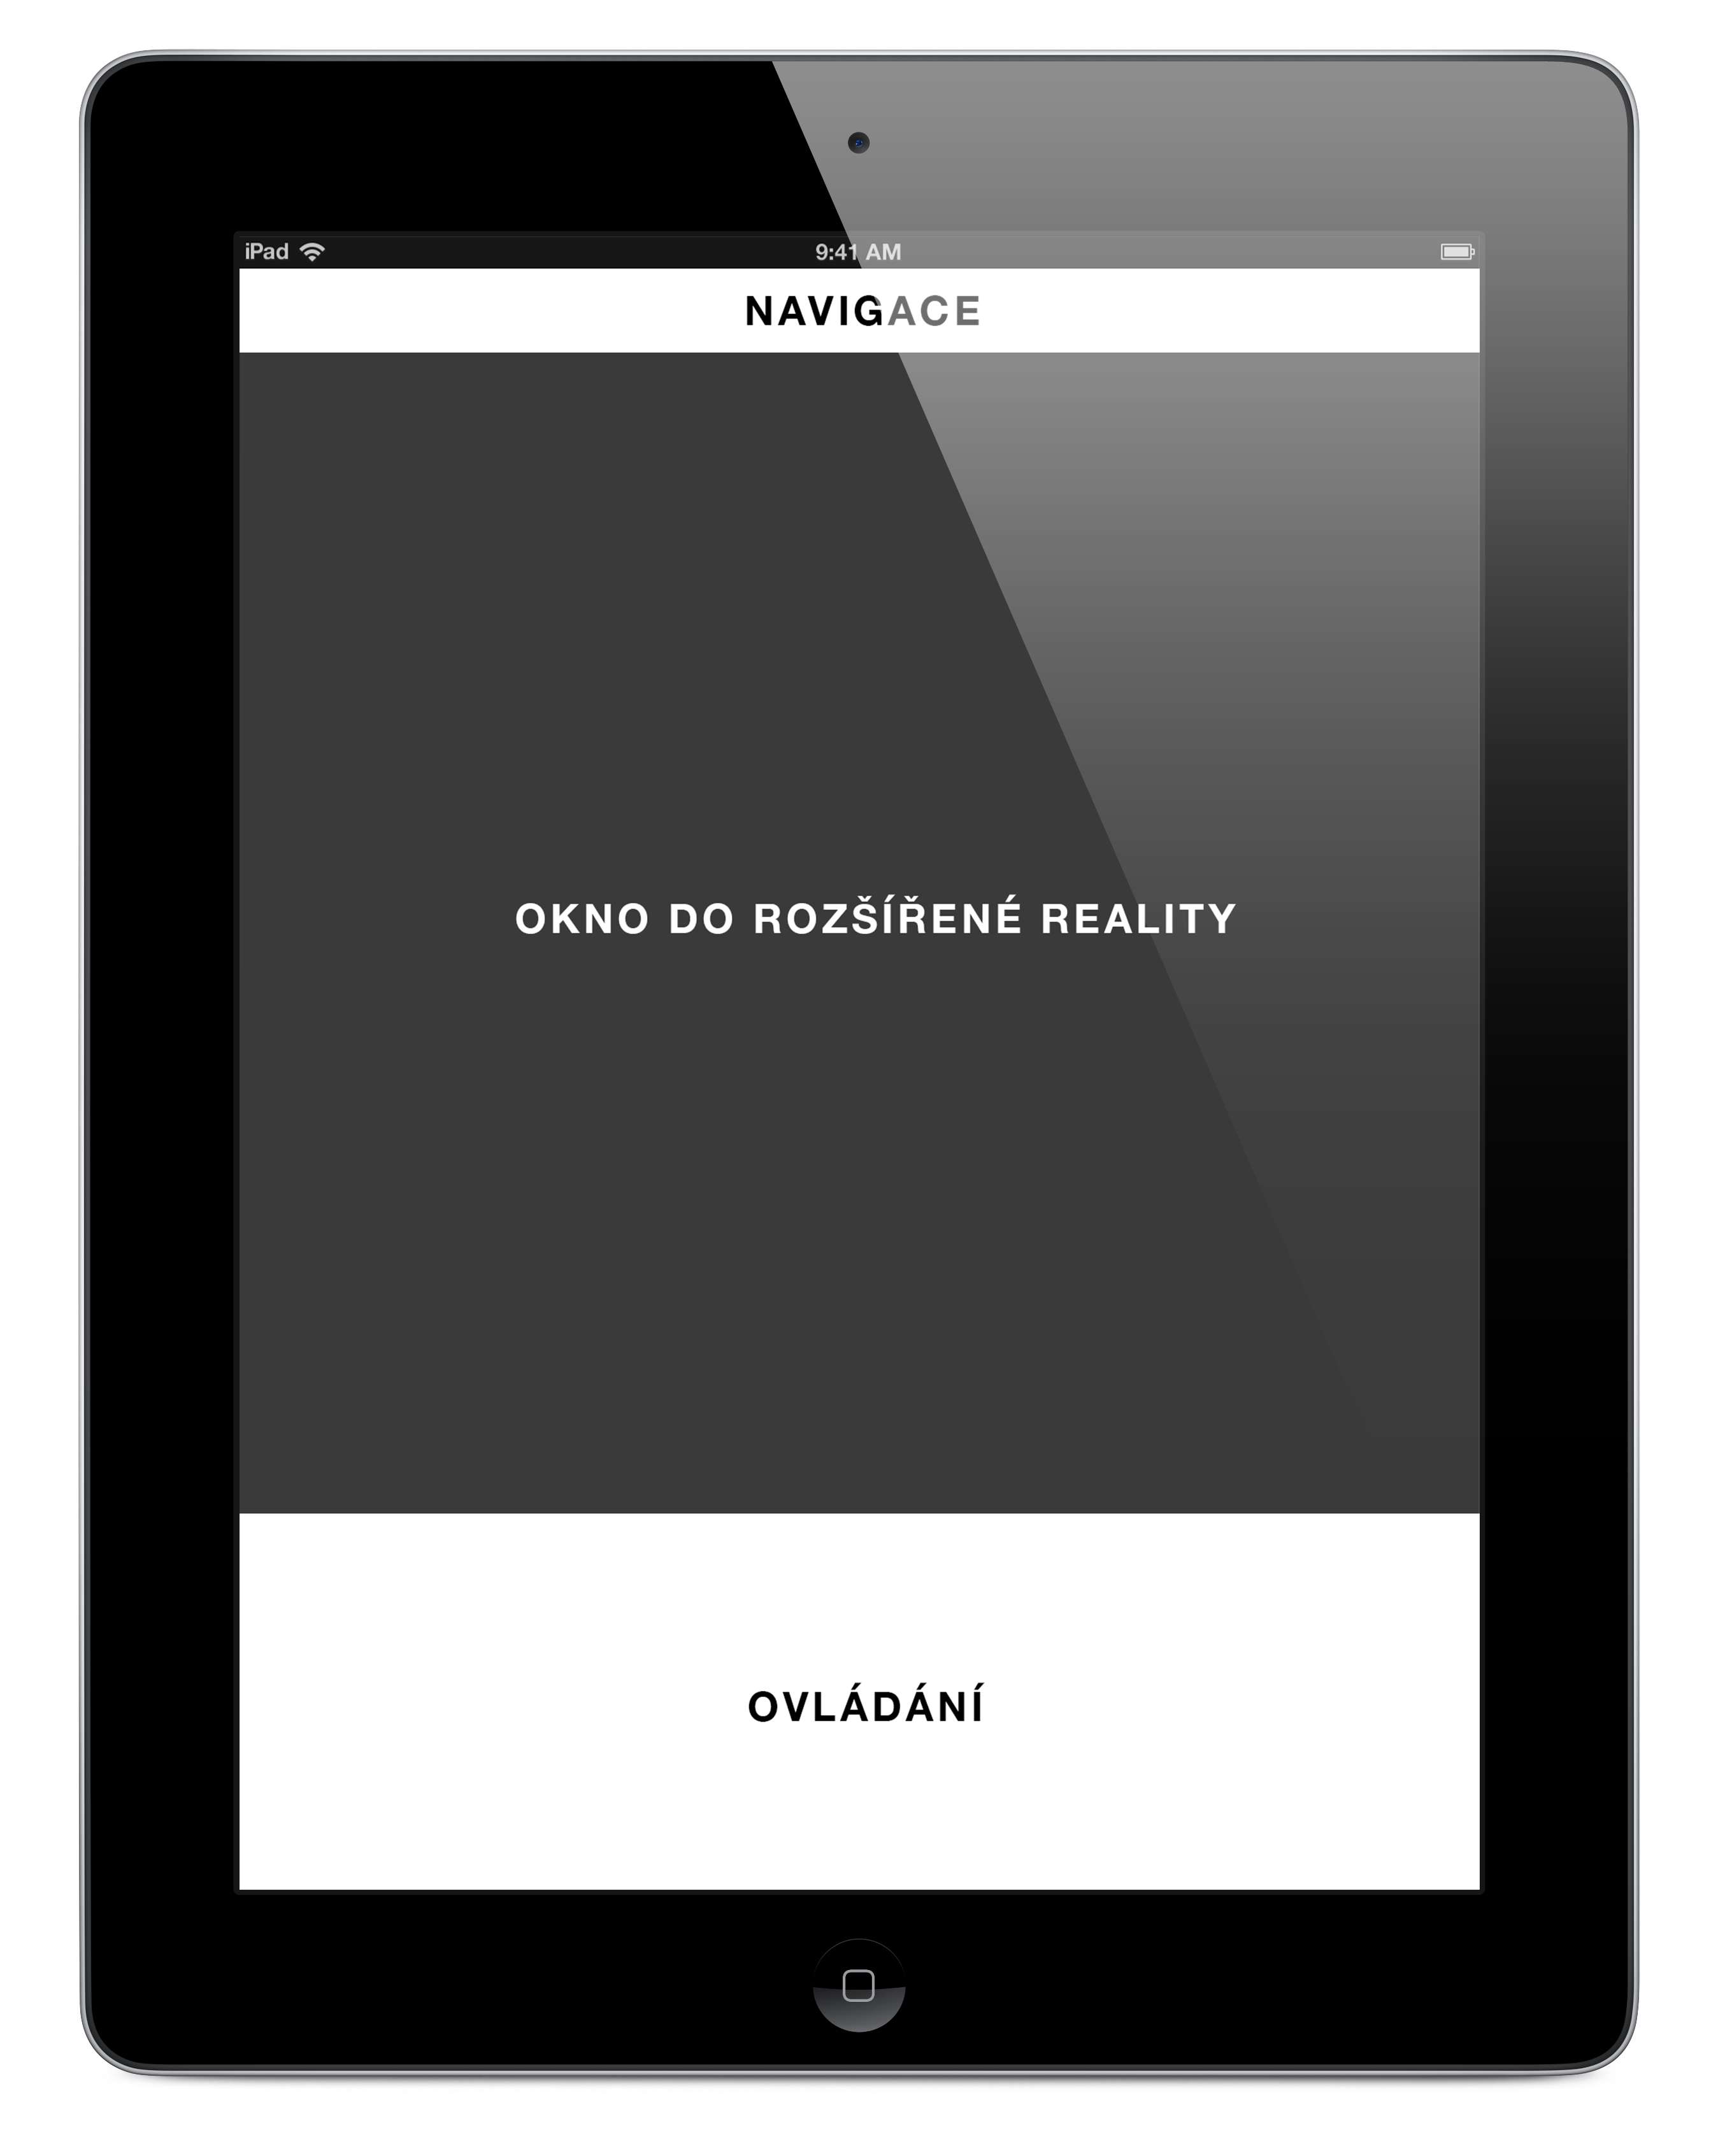
\includegraphics[width=300px, center]{images/ipad_layout_ux.jpg}
\captionsetup{justification=centering}
    \caption{Aleš Kocur, \textit{Výsledný návrh rozložení prvků pro hru ARCity}}
    \label{class_diagram}
\end{figure}

Z konceptu hry vyplývají 2 hlavní ovládací prvky. První umožňující stavbu zón a druhý zobrazení informací o vybrané postavené zóně s možností zónu vylepšit. Z tohoto předpokladu lze vyvodit, za jakých okolností je potřeba toto ovládání zobrazovat. V prvním případě je to když uživatel vybere práznou parcelu pro stavu zóny, v druhém pak při výběru nějaké konkrétní zóny. V kterémkoliv jiném případě není ovládací části potřeba a můžeme ji skrýt ve prospěch zvětšení plochy pro okno do rozšířené reality.

\newpage

\podsekce{Design}

Design je velmi subjektivní součást návrhu rozhraní a jeho líbivost není nikdy zaručena, protože je hodnocen subjektivně hodnotitelem na základě jeho vkusu. Nehledě na tuto skutečnost, měl by se design držet několika pravidel:

\begin{itemize}
\item Jednoduchost
\item Intuitivnost
\item Vypovídající o své funkci (tzv. self-explanatory)
\item Ohled na různá postižení (např. poruchy barvocitu) 
\end{itemize}

Na základě těchto pravidel byl navrhnut vysoce kontrastní, černobílý, design pro veškeré prvky, postavený na typografii použitím bezpatkového písma Helvetica Neue navrženého Maxem Miedingerem v řezech Light a Bold, doplněný o piktogramy vyjadřující povahu jednotlivých zón a statistik.  
 
 \begin{figure}[H]
\centering
    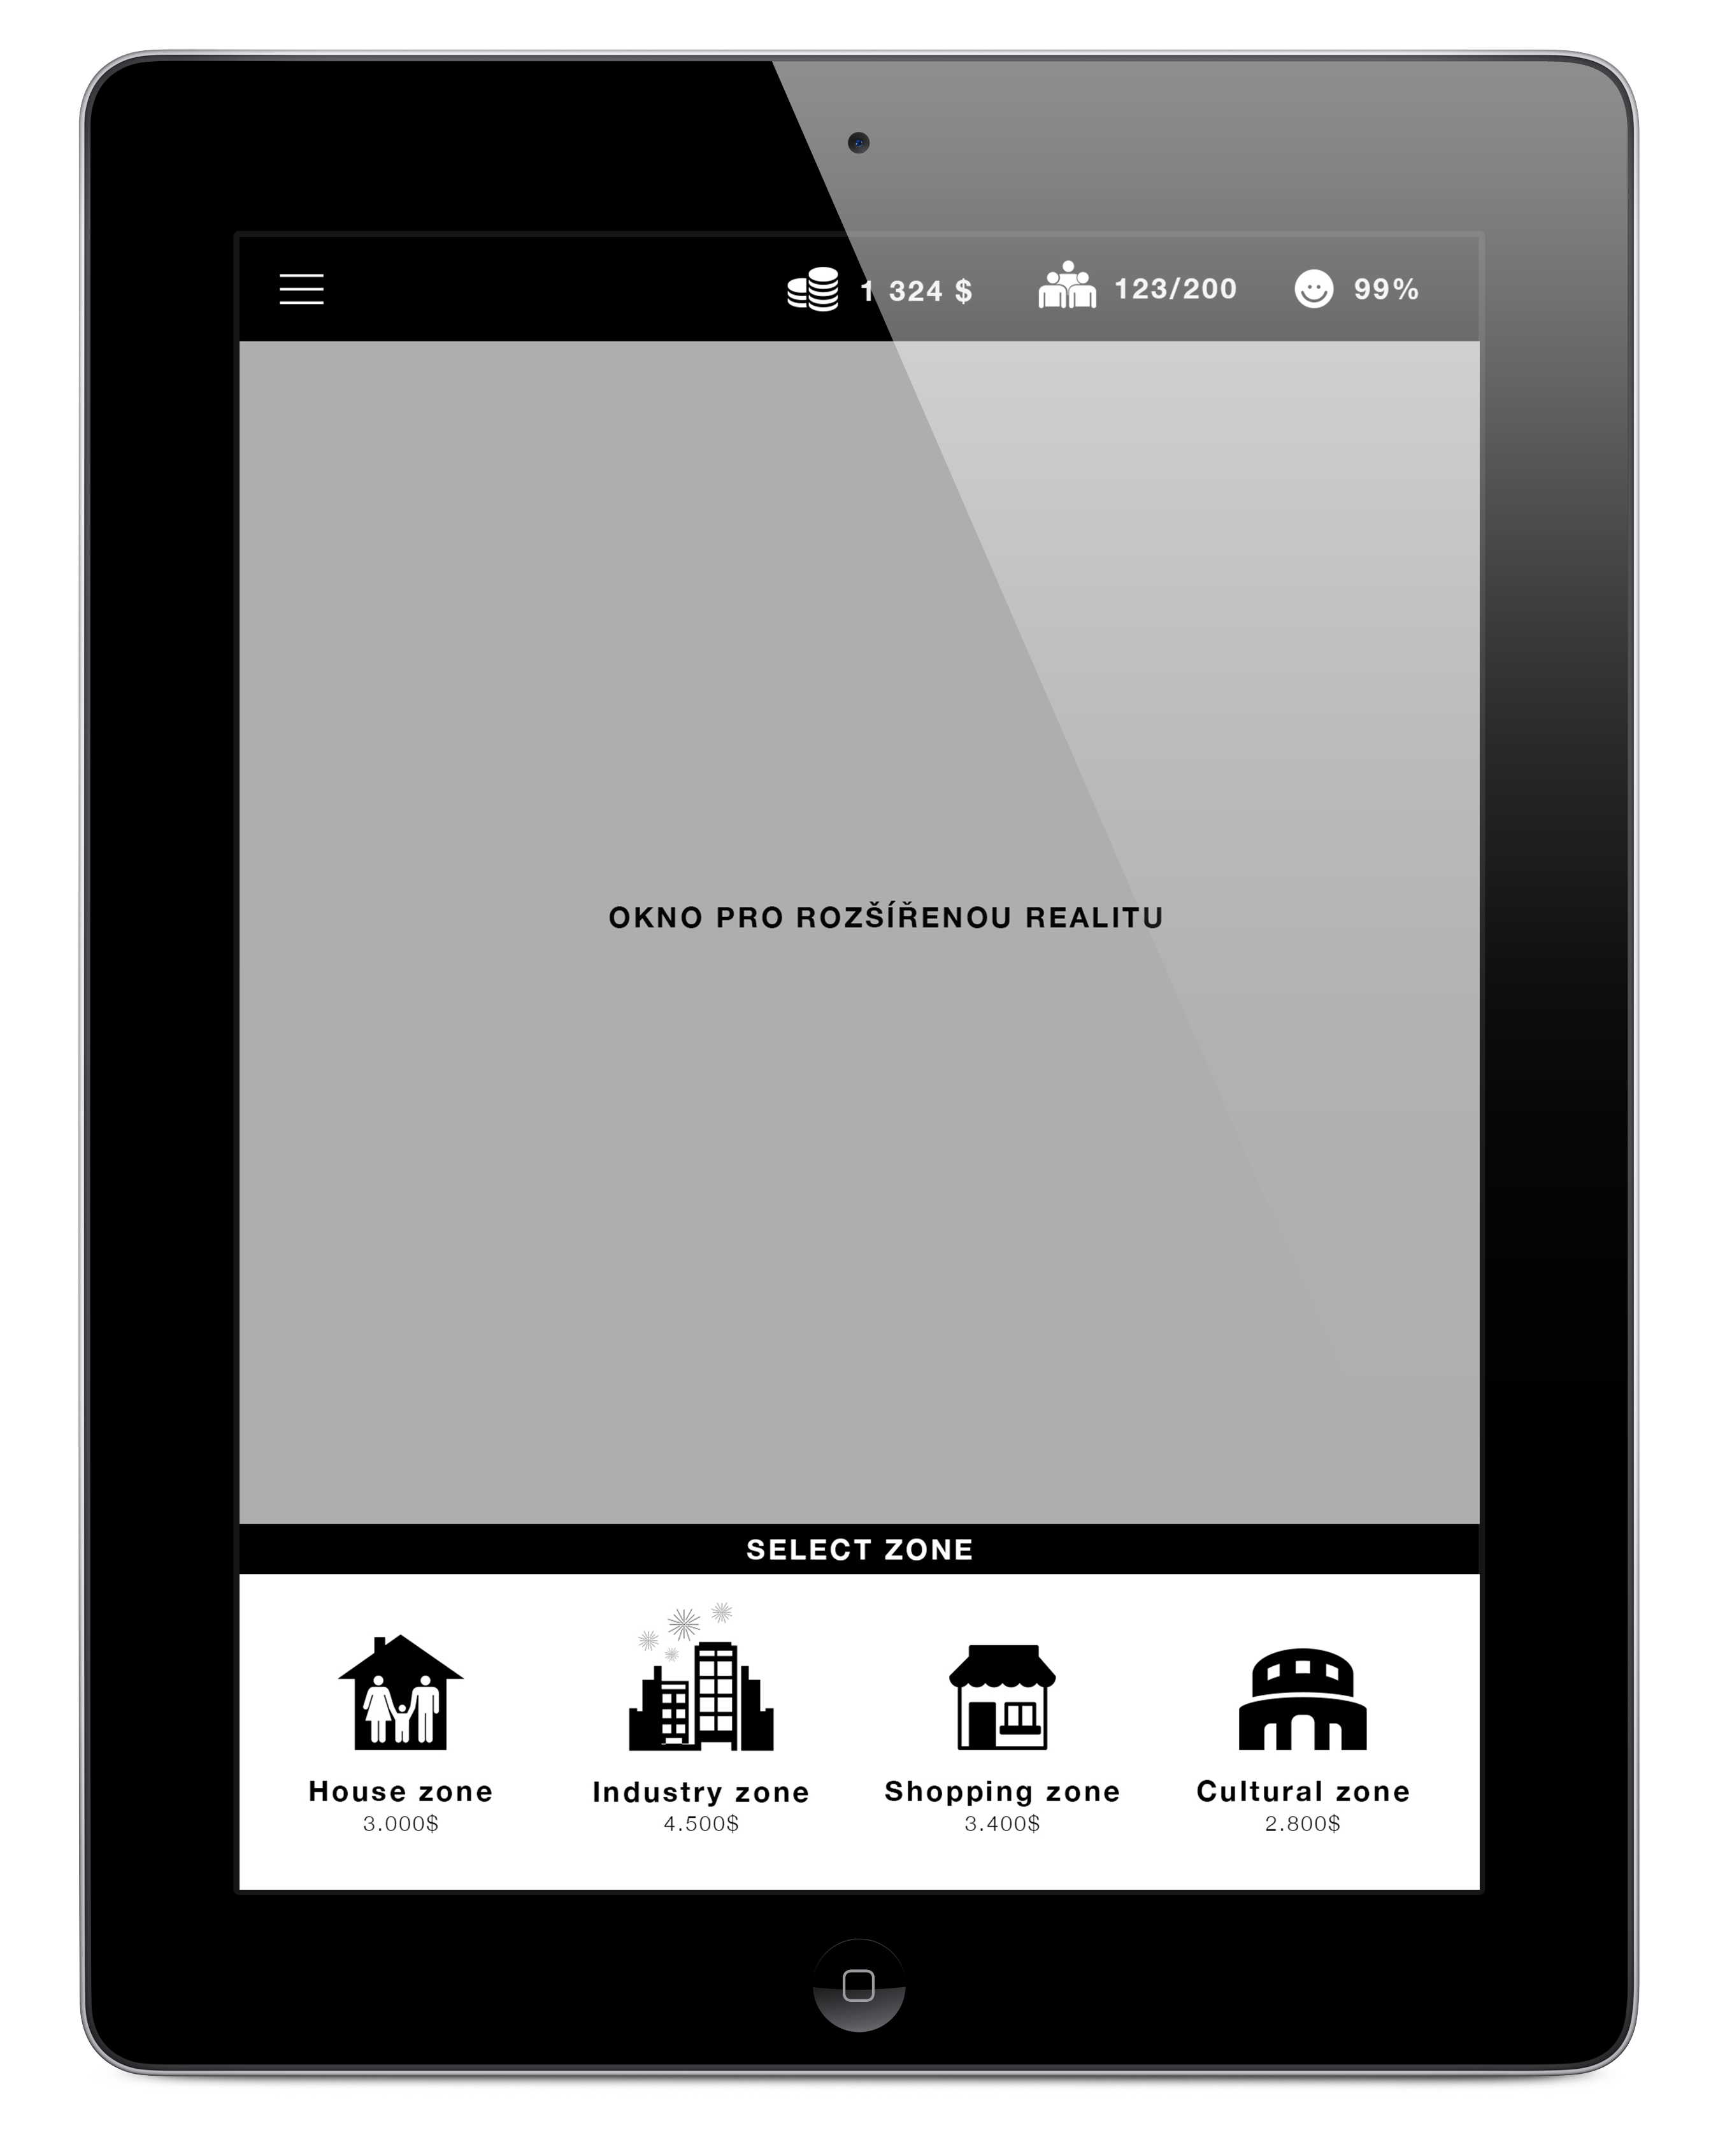
\includegraphics[width=430px, center]{images/ipad-layout.jpg}
\captionsetup{justification=centering}
    \caption{Aleš Kocur, \textit{Ukázka z grafického návrhu aplikace}}
    \label{class_diagram}
\end{figure}
 
 \sekce{Ukládání dat}
 
 Hra využívá pro ukládání dat zmíněný MagicalRecord framework, který obaluje systémovou knihovnu zvanou Core Data. Návrh datového modelu vychází z UML diagramu tříd ukládané části -- GameSession, Plot, Zone a Player.
 
 \begin{figure}[H]
\centering
    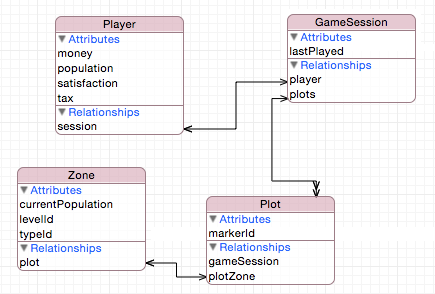
\includegraphics[width=400px, center]{images/core-data-model.png}
\captionsetup{justification=centering}
    \caption{Aleš Kocur, \textit{Datový model hry ARCity}}
    \label{class_diagram}
\end{figure}

 \sekce{Výpočty ukazatelů}
 
 Hra pracuje s pěti typy ukazatelů stavu hry:
  
 \begin{itemize}
\item Peníze
\item Populace (aktuální/maximální)
\item Spokojenost obyvatel
\item Pracovní místa
\item Daň
\end{itemize}
 
 Ukazatel typu Peníze stojí na jednoduchém principu přičítání a odečítání hodnot stanovených jako cena za stavbu/vylepšení/provoz. Stejně tak maximální hodnota populace je součet postavených obytých zón respektive jejich kapacit, které se odvíjí od jejich úrovně vylepšení. Změna těchto hodnot probíhá právě při zmíněných úkonech -- stavba, vylepšení, provoz budovy. Na stejném principu funguje i výpočet počtu pracovních míst.
 
 Dalšími typy ukazatelů jsou aktuální stav populace a spokojenost. Tyto hodnoty jsou vypočítávány v pravidelných intervalech a jsou ovlivňovány více aspekty. Rychlost iterace těchto výpočtů stanovuje rychlost hry a na základě několika zkoušení byl jako ideální interval stanoven na 3 sekundy. Obecný princip výpočtu hodnot spočívá v nalezení nové hodnoty na základě parametrů příslušných danému ukazateli. Odečtením aktuálního stavu od této nové, očekávané hodnoty, zíkáme rozdíl mezi puvodním stavem a novým stavem a ten je vynásoben nějakou malou konstantou pohybující se kolem 0,5 a přičten k původnímu stavu. Tímto nám hodnoty např. po stavbě zóny přidávající spokojenost nevystoupají hodnoty skokově, nýbrž parabolicky během několika iterací.
 
 Jako příklad uveďme počáteční stav spokojenosti 20 \%. Po stavbě kulturní zóny v první iteraci vypočteme novou hodnotu -- 60 \%.  Od nové hodnoty odečteme původní a získáme rozdíl: 
 
 $$ 0,6 - 0,2 = 0,4 $$
 
 Tento rozdíl je vynásoben číslem 0,5.
 
 $$ 0,4 \times 0,5 =  0,2 $$
 
 Přičtením k původnímu stavu dostáváme nový stav po první iteraci -- 40 \%. Stejným způsobem v dalších iteracích dostaneme nové hodnoty 50 \%, 55 \%, 57 \%, 58 \%, 59 \% a 60 \%. Celkový čas do stabilizace ukazatele lze pak vypočítat podle vzorce:
 
 \begin{equation}
t = h \times d
\end{equation}
 
 kde $t$ je výsledný čas, $h$ je počet hodnot resp. iterací a $d$ je délka trvání iterace v sekundách.
Dozasením dostaneme výsledek v podobě délky trvání stabilizace a to 21 sekund.
 
 Konkrétní vzorec pro každý ukazatel je navrhnut na jeho logické návaznosti k ostatním ukazatelům a ovlivňují se tudíž navzájem. Po každé změně ve hře následuje stav postupné stabilizace. Po několika iteracích se ukazatele hry stabilizují na určitou hodnotu. Pravidla pro výpočty zbylých ukazatelů jsou definovány těmito vzorci.
 
 \podsekce{Počet obyvatel}
 
 \begin{equation}
p = mp \times s
\end{equation}
 
 kde $p$ je populace, $mp$ je maximální možná populace a $s$ je spokojenost.
 
\podsekce{Spokojenost}

\begin{equation}
s = \frac{f(o,m) + f(o, sz) + g(dk, d)}{3}
\end{equation}

kde

\begin{equation}
f(x, y) = \left\{
  \begin{array}{lr}
     \frac{y}{x} & : x > y\\
    1,0 & : jinak
  \end{array}
\right.
\end{equation}

\begin{equation}
g(x, y) = \left\{
  \begin{array}{lr}
     1,0 & : \frac{y}{x} - 0,5 > 1,0\\
     0 & : \frac{y}{x} - 0,5 < 0\\
    \frac{y}{x} - 0,5 & : jinak
  \end{array}
\right.
\end{equation}


a $o$ je aktuální počet obyvatel, $m$ je počet pracovních míst, $sz$ je hodnota uspokojení z dosud postavených zón, $dk$ je konstanta pro průměrnou daň a $d$ je aktuální daň.

\kapitola{Ukázky z práce}

\begin{figure}[H]
\centering
    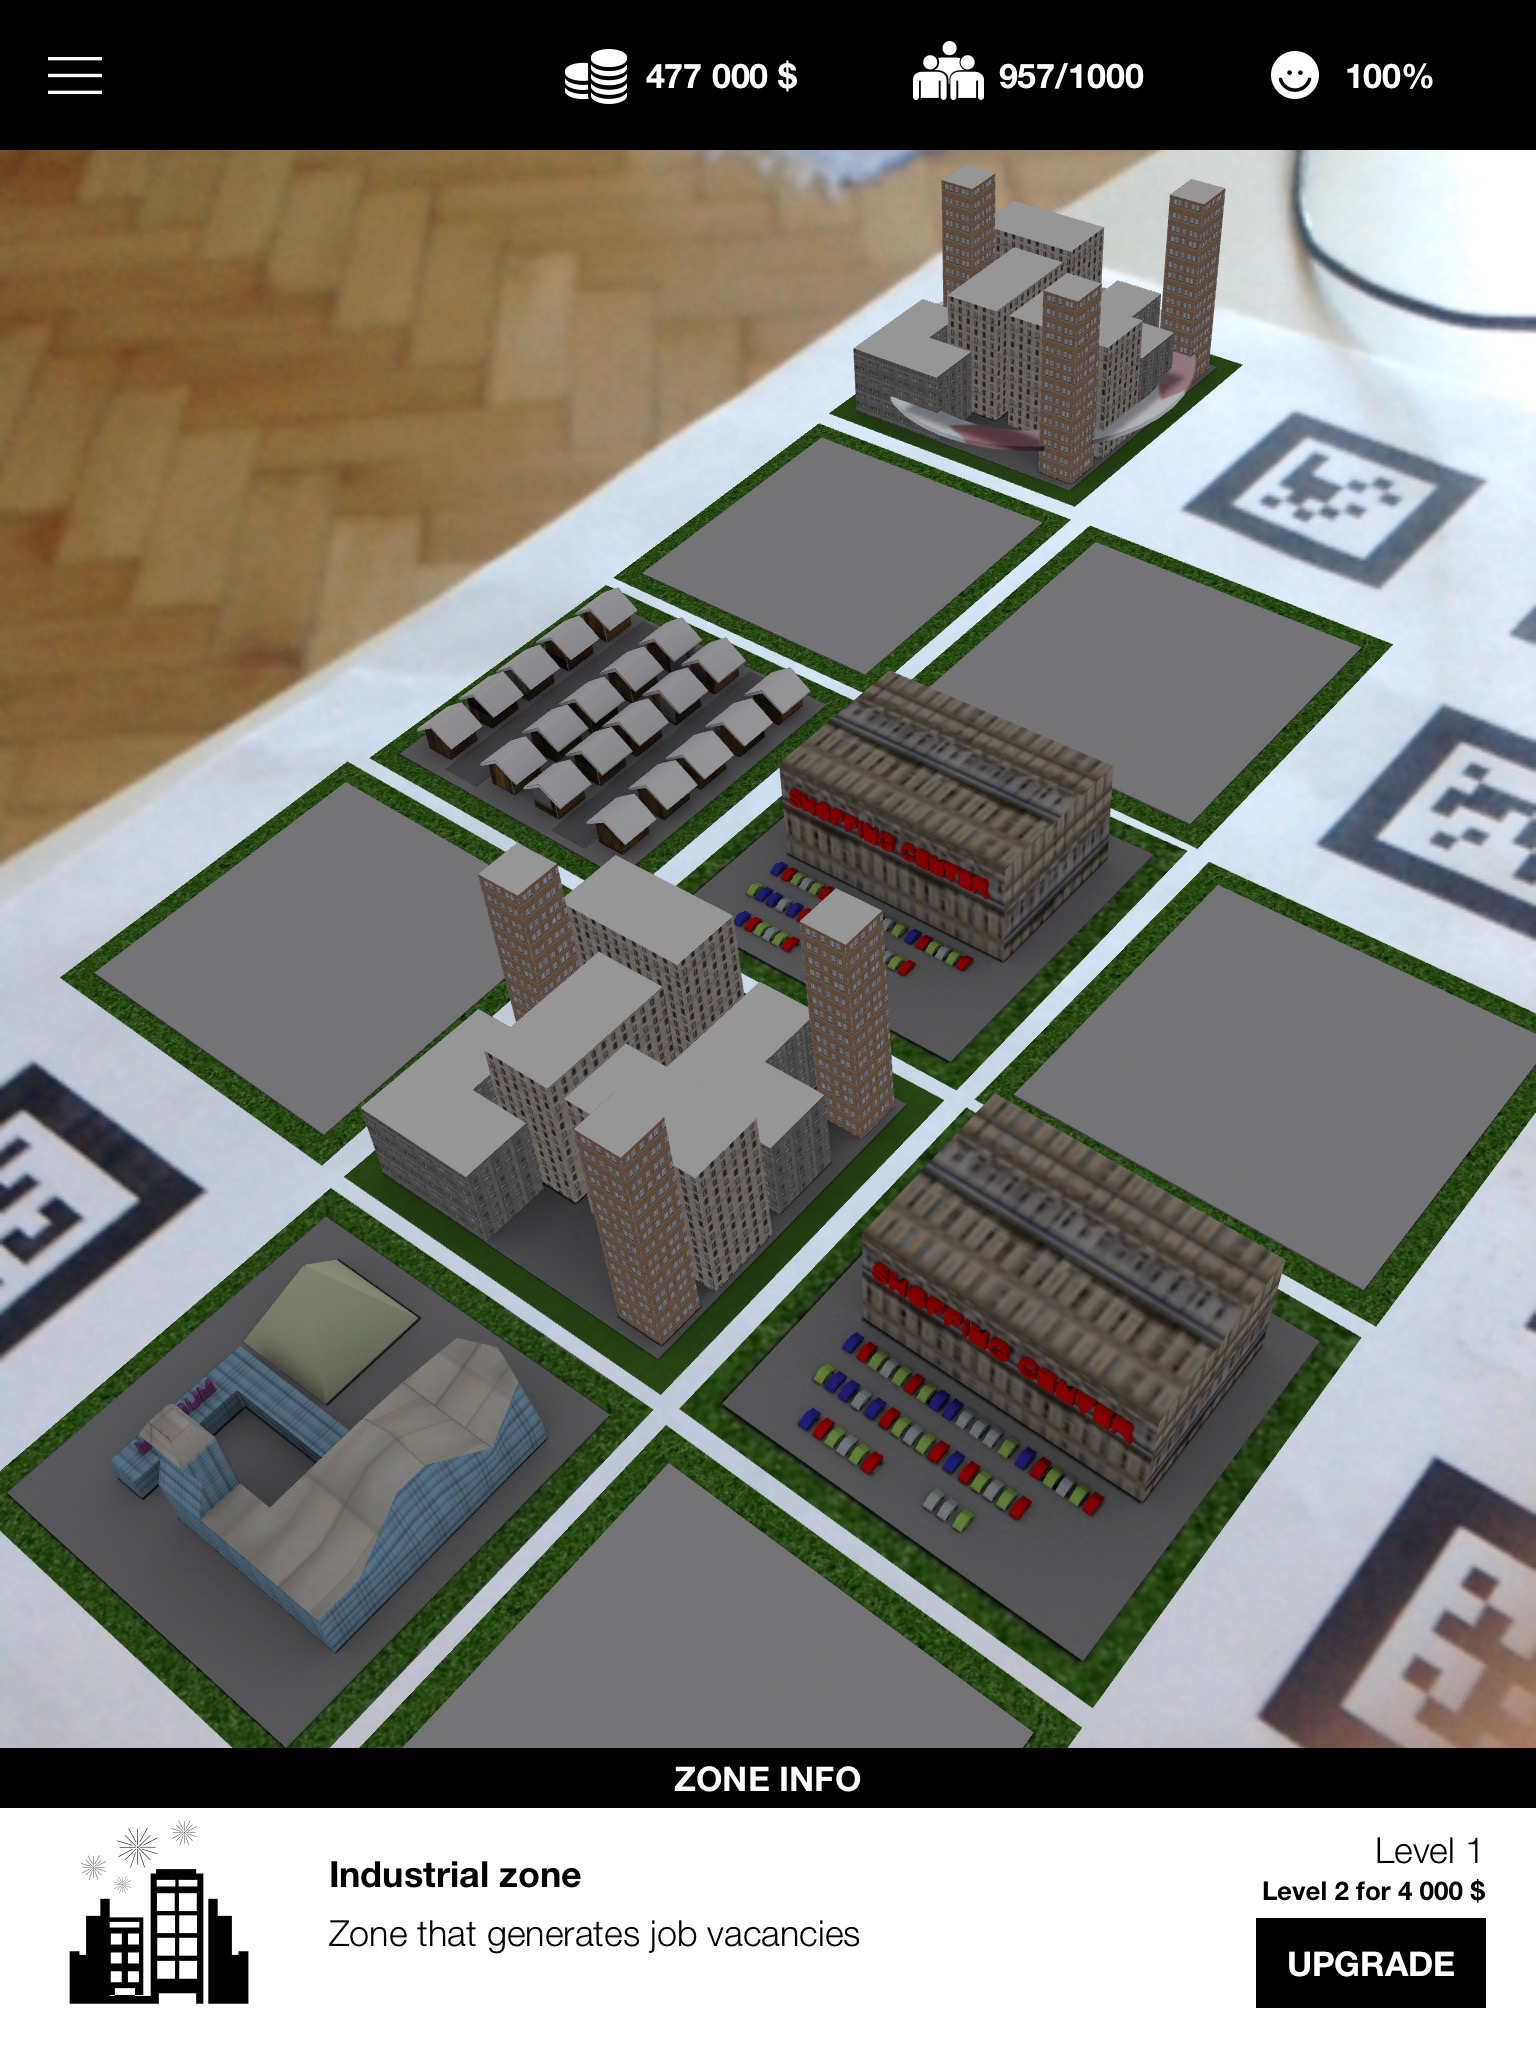
\includegraphics[width=400px, center]{images/screenshot1.jpg}
\captionsetup{justification=centering}
    \caption{Aleš Kocur, \textit{Screenshot ze hry ARCity}}
    \label{screenshot3}
\end{figure}

\begin{figure}[H]
\centering
    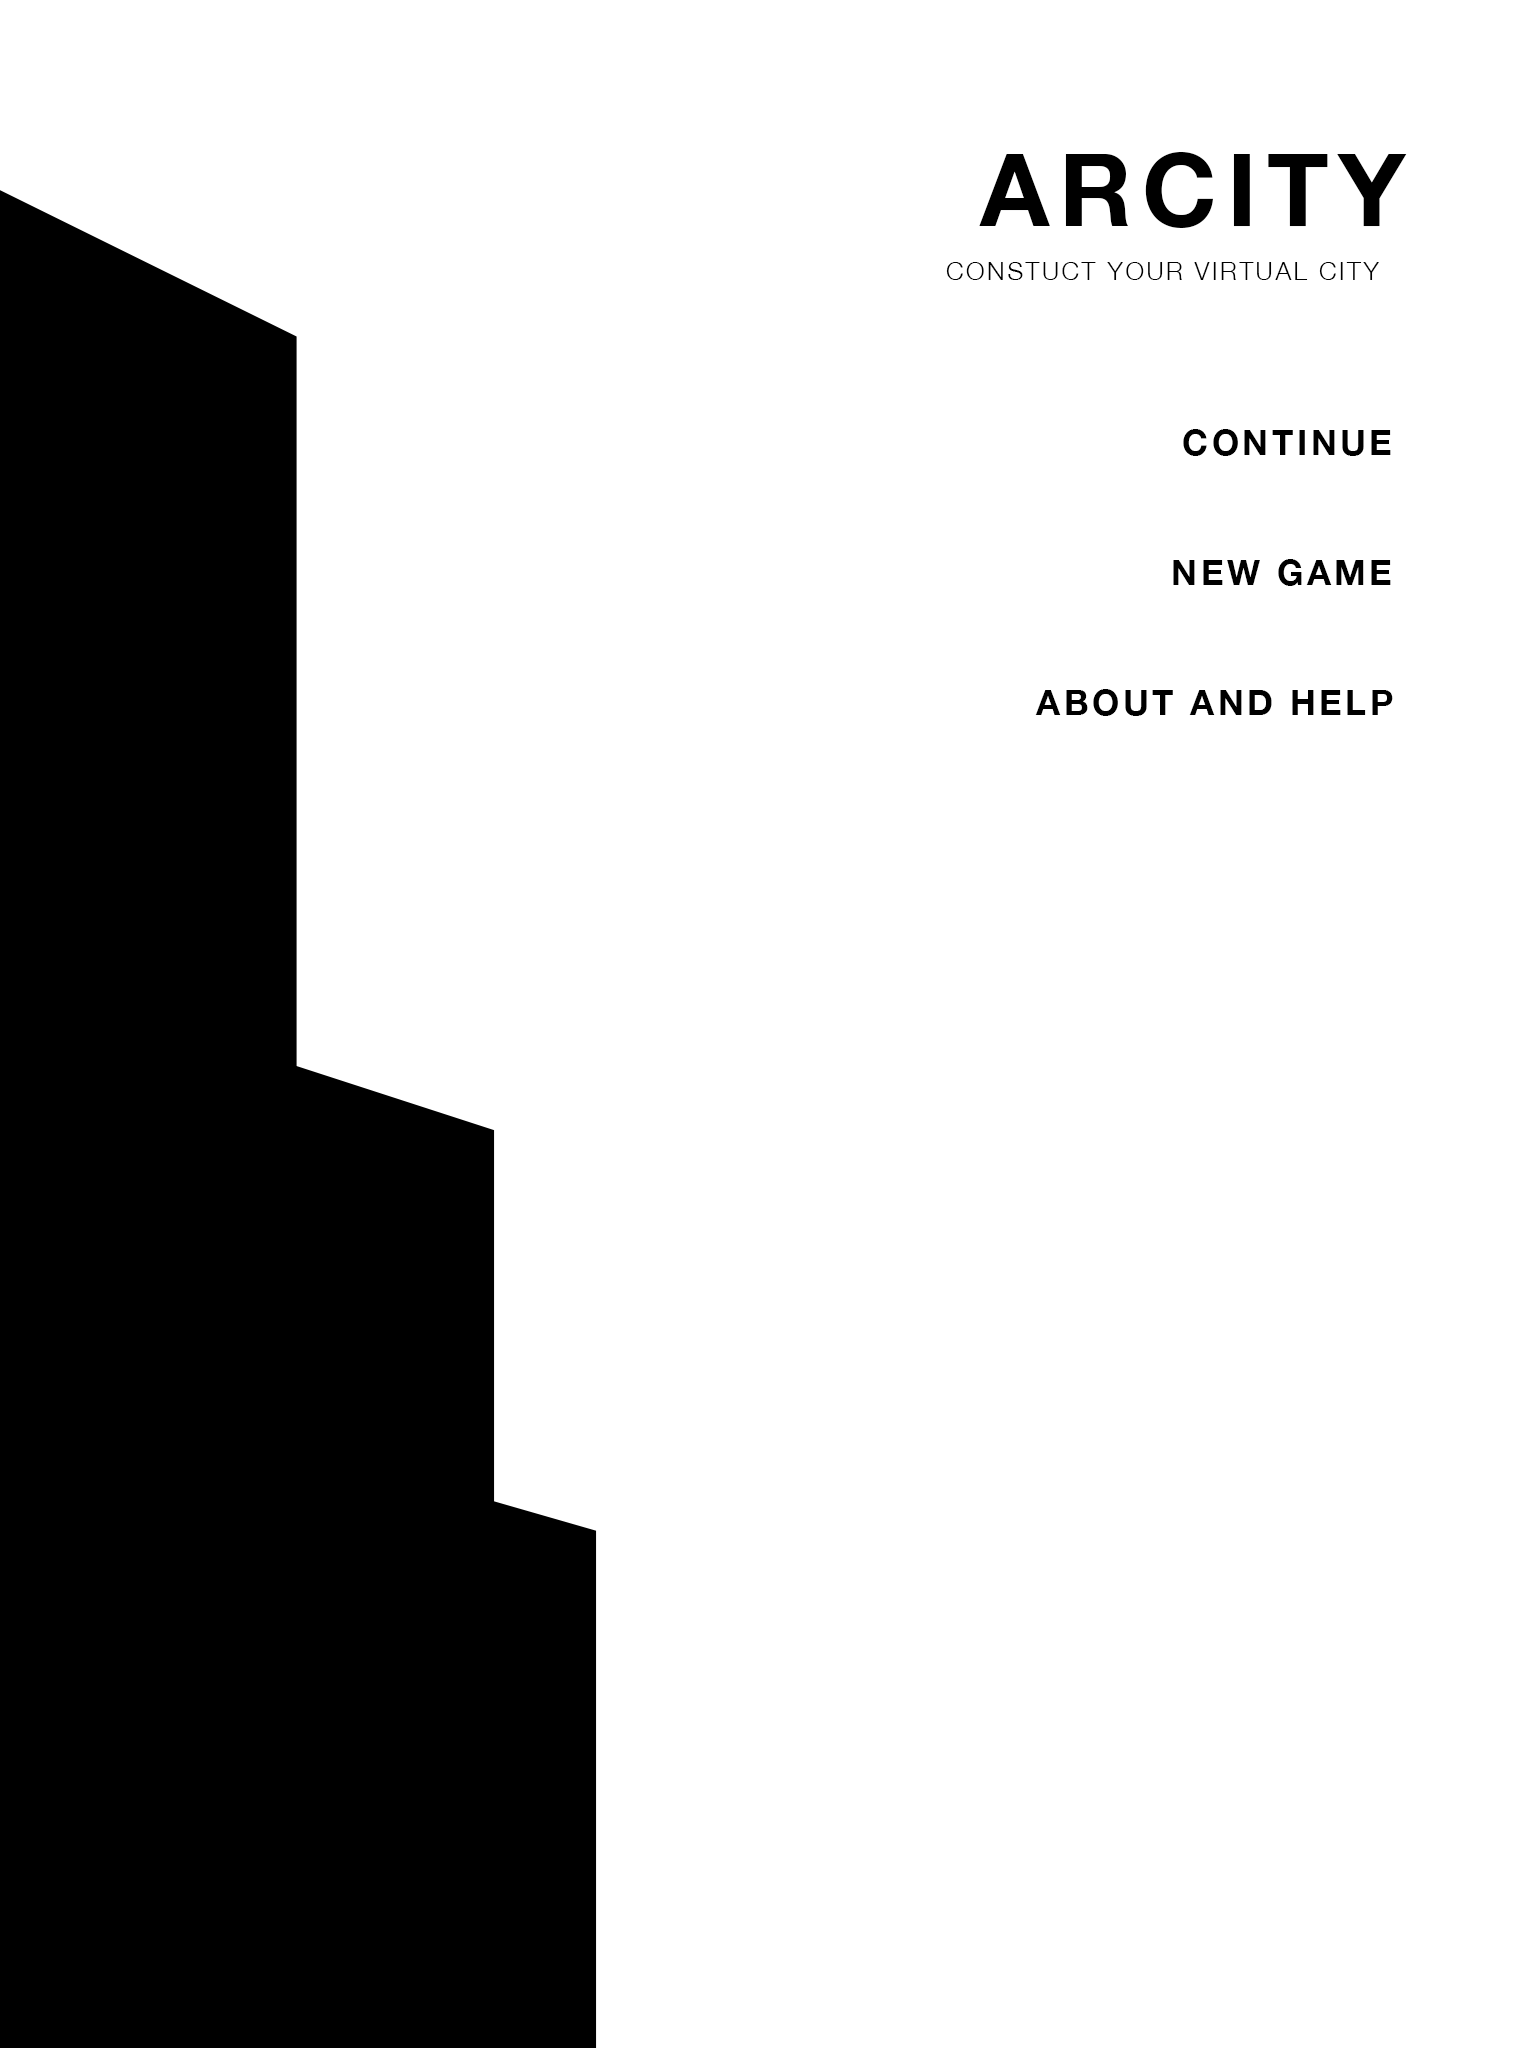
\includegraphics[width=400px, center]{images/screenshot2.png}
\captionsetup{justification=centering}
    \caption{Aleš Kocur, \textit{Hlavní menu ze hry ARCity}}
    \label{screenshot3}
\end{figure}

\begin{figure}[H]
\centering
    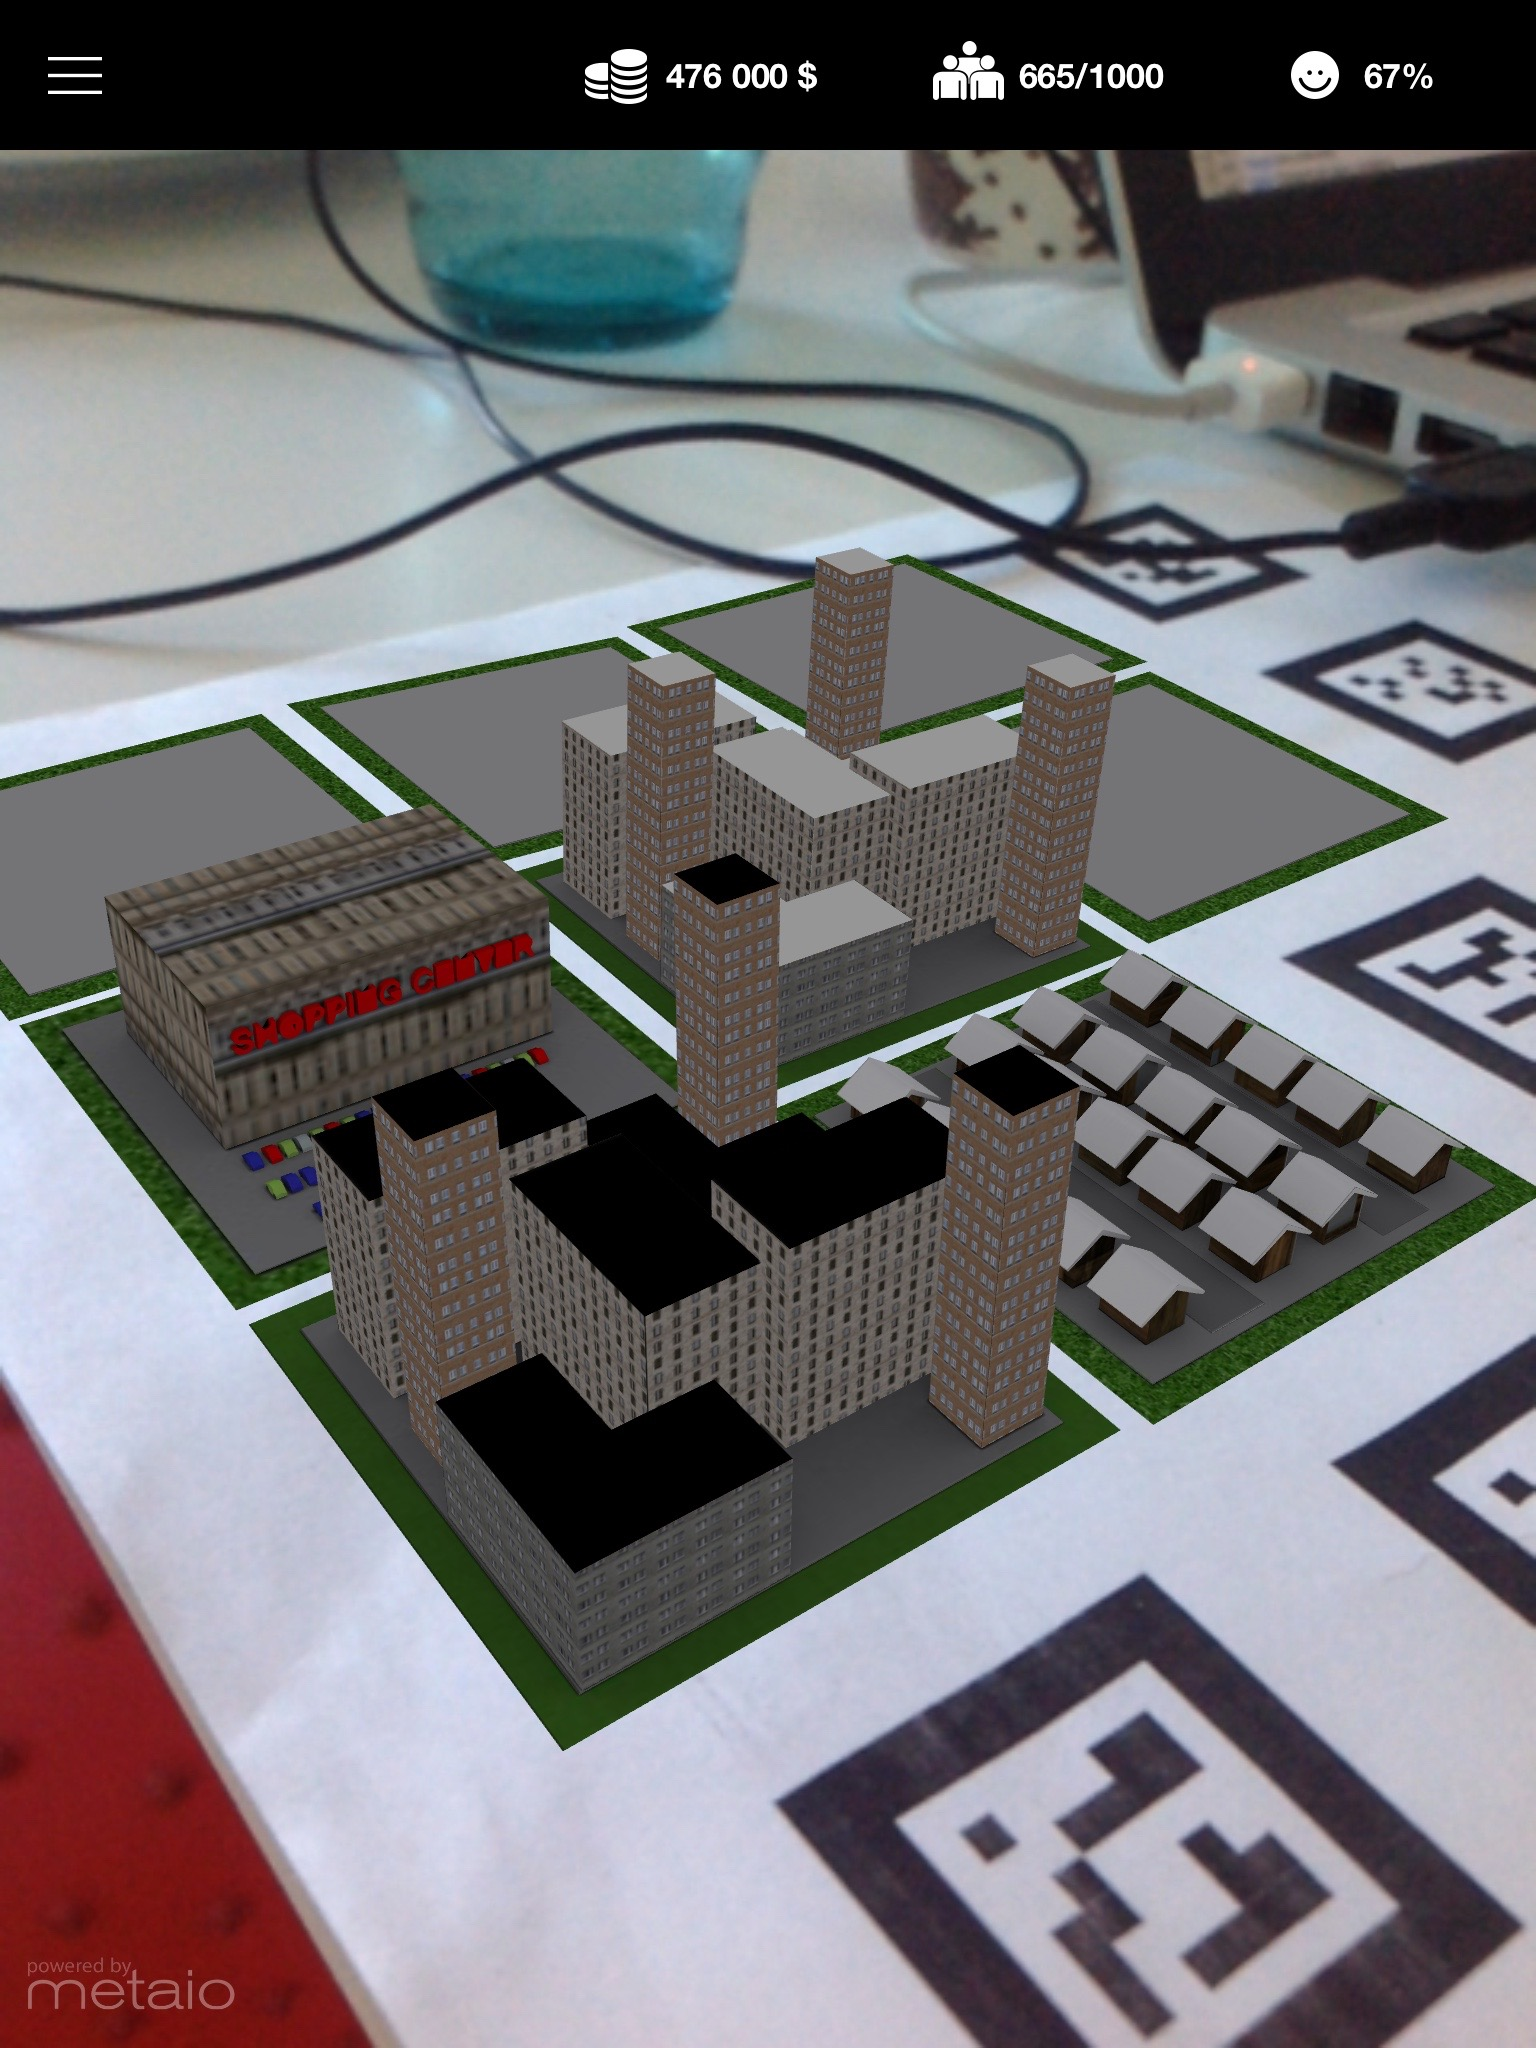
\includegraphics[width=400px, center]{images/screenshot3.jpg}
\captionsetup{justification=centering}
    \caption{Aleš Kocur, \textit{Screenshot ze hry ARCity}}
    \label{screenshot3}
\end{figure}


\newpage

\kapitola{Testování uživatelského rozhraní}
Jedním z pilířů použitelnoti je uživatelské testování. Mnoho skutečností, které programátor či designér aplikace považují za samozřejmé, nemusí být pro uživatele na první pohled patrné či srozumitelné. Steve Grug, autor knihy \textit{Nenuťte uživatele přemýšlet!: praktický průvodce testováním a opravou chyb použitelnost webu}, přirovnává uživatelské testování k návštěvě cizinců v rodném městě. Provádíme-li je po svém městě, všimneme si věcí, které jsme doposud nevnímali, protože jsme je brali jako samozřejmost \cite{krug_steve}.

\sekce{Základní přístupy testování}
Existují různé přístupy, jak lze uživatelské testování provádět. Liší se zejména v časové a technologické náročnosti. Vhodný typ testování je nutno zvolit na základě projektu, který má být testován. 

\podsekce{Eye tracking}
Jedná se o velmi populární metodu snímání uživatelského zacházení s produktem. K testování je potřeba člověka-testera, který bude daný produkt používat, a to nejlépe bez předchozí zkušenosti. Při testování se sledují pohyby očí v poměru k obrazovce a získáváme tím obraz uživatelova zájmu. Více porozované oblasti pak lze odlišit barvami a získáme pro jednotlivé obrazovky zóny největšího soustředění uživatelova zraku. Analýzou těchto dat pak můžeme zlepšit umíštění důležitých ovládacích prvků do zón s vysokým indexem soustředění, případně se změnou barevnosti a kontrastu pokusit tyto zóny přemístit. Ke snímání soustředěnosti zraku uživatele-testera je možno použít speciálních brýlí či helem. Toto řešení je nicméně nákladnější na počáteční nákup hardwaru a softwaru a proto vznikly alternativy. Tou je například pro testování mobilních aplikací metoda využití přední kamery pro snímání místa pozorování. Uživatelé-testeři jsou snímáni přímo zařízením během procesu testování a pozorovací mapy jsou generovány přímo pro konkrétní obrazovky, na kterých se právě tester nachází. Eye tracking lze samozřejmě využít i k jiným věcem než k uživatelskému testování, důkazem může být například firma uMoove vyvíjející SDK pro interakci s aplikacemi pomocí eye trackingu \cite{umoove}.

\podsekce{Heuristic evaluation}
Heuristická analýza uživatelského přístupu spočívá v prozkoumání uživatelského rozhraní a kontrole nedostatků na základě zkušeností. Zkušenostmi máme na mysli seznam poznatků, které by neměly být při návrhu rozhraní opomenuty. Výhoda tohoto testování je, že není potřeba uživatele-testera, ale tento test může být vyhodnocen kýmkoliv kompetentním v daném projektu. Zkoumáním lze pak například zjistit, že v některých situací uživatel ztrácí přehled o aktuálním stavu aplikace nebo nemá možnost návratu k přechozím stavům aplikace. Jedním ze zakladatelů tohoto přístupu je Jakob Nielsen, který vytvořil jakési desatero základních principů pro interaktivní design (překlad \cite{lichnovskakarberova}, originál \cite{nielsen}): 

\begin{enumerate}
\item Viditelnost stavu systému
\item Spojení mezi systémem a reálným světem
\item Uživatelská kontrola a svoboda
\item Konzistence a standardizace
\item Prevence chyb
\item Rozpoznání místo vzpomínání
\item Flexibilní a efektivní použití
\item Estetický a minimalistický design
\item Pomoc uživatelů poznat, pochopit a vzpamatovat se z chyb
\item Nápověda a návody
\end{enumerate} 

Zamyšlením se nad těmito body v kontextu dané aplikace můžeme objevit její nedostatky.

\podsekce{Focus Groups}
Hlavní podstatou tohoto testování je doplnění informací o použitelnosti, zejména pak uplatnění některých funkcí. Testování je vedeno formou diskuze ve skupině několika lidí, nejlépe různých postavení, zájmů a pohlaví. Diskuzi vede moderátor a jeho hlavním úkolem je udržovat či překlánět diskuzi k potřebným tématům. Úskalím této medoty může být výskyt dominantního člena diskuzní skupiny, který následně strhává názory ostatních \cite{nielsen_focus_groups}.

\podsekce{Cognitive walkthrough}
Česky tzv. Kognitivní průchod je způsob testování uživatelského rozhraní za pomocí testerů, kteří zkoumají složitost průchodu aplikací s daným účelem. Testerem zde může být jak člověk nepodílející se na přímo na vývoji aplikace tak i naopak. Jako příklad průchodu lze uvést registraci, přihlášení a také specifické průchody typu rezervace v rezervačním systému a podobně. Takto se stanoví průchody a cíle pro danou aplikaci. V průchodu je hodnocena jednoduchost (počet akcí uživatele nutných k průchodu), intiutivnost (srozumitelnost informací), navigace (možnost návratu z nevyžádaných pozic). Při nalezení nedostatu při průchodu je zaznamenán a označen prioritou, podle které je mu pak nutno věnovat resp. nevěnovat pozornost. 

\podsekce{Další metody a shrnutí}
Metod testování uživatelskéro rozhraní je velmi mnoho. Za zmínku stojí dále také \textit{Formal usability inspections}, \textit{Pluralistics walkthroughs}, \textit{Feature inspection}, \textit{Consitency inspection} a \textit{Standard inspection}, a informace o nich lze nalézt v rešerši \textit{Usability Inspection Methods} napsané roku 1994 \textit{Jakobem Nielsenem} \cite{nielsen_methods}. 

Pro testování této aplikace jsem zvolil metodu heuristické analýzy a to hlavně z důvodu možnosti testování mnou samým.

\sekce{Heuristická analýza ARCity}
Na základě uvedených informací bylo sepsáno 10 bodů odpovídající desateru základních principů popsaných v sekci \textit{Základní přístupy testování - MetodyHeuristic evaluation} a posouzeno v kontextu této aplikace.

\podsekce{Viditelnost stavu systému}
Této viditelnosti je dosaženo statickým umístěním ukazatelů hry do horní části obrazovky. Uživatel má v každém daném stavu hry možnost zjistit v jakém stavu se jeho město nachází (počet obyvatel, stav peněz, spokojenost, počet pracovních míst).

\podsekce{Spojení mezi systémem a reálným světem}
Veškeré texty jsou psány srozumitelně a výstižně. Některé důležité prvky doplňují pikrogramy pro ještě větší srozumitelnost na první pohled. Nevyskytují se zde žádné odborné termíny.

\podsekce{Uživatelská kontrola a svoboda}
Umístěním tlačítka pro menu v horním levém rohu má uživatel možnost kdykoliv hru pozastavit. Stejně tak při minimalizaci je aplikace automaticky ukládána a její případná terminace nemá následek na poslední stav hry. Možnost odvolání akcí při stavbě města není v učividných důvodů žádoucí.

\podsekce{Konzistence a standardizace}
Hra se drží standardních termínů pro zahájení hry (\textit{angl. New game}) či pokračování (\textit{angl. Continue}). Stejně tak zavádí názvy jednotlivých zón a tyto názvy jsou použity napříč celou aplikací při jejich zmínce.

\podsekce{Prevence chyb}
Design aplikace dovoluje uživateli provádět pouze platné tahy. Nemůže například nastat situace kdy při označení již postavené zóny by se uživateli zobrazilo menu pro stavbu nové zóny nebo opačně při označení prázdné parcely zobrazení menu s detaily a možností vylepšení. 

\podsekce{Rozpoznání místo vzpomínání}
Zobrazením menu s akcemi přesně ve chvíli kdy uživatel označí položku je pro uživatele snadno rozpoznatelným impulsem očekávajícím jeho reakci ve smyslu volby. Naopak jeho skrytím kdy volba není potřeba je upřednostněno místo pro herní plochu a tím vybízeno k provedení akce na herní desce.

\podsekce{Flexibilní a efektivní použití}
Náročnější uživatelé mají možnost jednoduše rozšířit herní plochu o další volné parcely přídáním až dvou dalších kopií herní plochy.

\podsekce{Estetický a minimalistický design}
Design je velmi minimalistický, kontrastní -- využívá pouze kombinace černé a bílé barvy -- a doplněn piktogramy, korespondující s černobílým designem. Snaží se vyjádřit přesnou podstatu každého užitého prvku.

\podsekce{Pomoc uživatelů poznat, pochopit a vzpamatovat se z chyb}
Rozsah chyb je natolik eliminován designem aplikace, že prosto zbývá pouze pro neidentifikovatelné chyby a kritické chyby kódu. V prvním případě se jedná o chybu kdy nejsou načteny textury objektů a tento stav je bohužel chybovým stavem použitého SDK a to nenabízí možnost jej ošetřit. V druhém pak končí chyba pádem aplikace. Všechny pády aplikací vypadají na iOS platformě stejně a uživateli je jasné, že je nutné aplikaci pustit znovu. Těmto chybám lze předejít pouze testováním kódu aplikace. Tento bod lze označit jako bod s nízkou prioritou pro vyřešení.

\podsekce{Nápověda a návody}
V menu má člověk přístupem na položku About and help možnost nechat si zobrazit základní informace o aplikaci, herní logice a jak s aplikací pracovat.

\sekce{Zhodnocení}
Na základě heuristické analýzy jsme došli k poznatku, že aplikace vyhovuje všem zmíněným bodům analýzy, pouze u předposledního bodu týkajícího se chybových stavů jsme zaznamenali drobný problém. Ten má však malou prioritu hlavně z důvodu velmi malé četnosti výskytu a také v podstatě nemožnosti opravy tohoto problému. 

Pro důkladnější hodnocení bychom mohli provést také Focus group metodu pro vylepšení hratelnosti a názory samotných hráčů. Správným řízením směřování diskuze bychom také mohli získat cenné nápady na budoucí vylepšování hry, případné přidávání nových zón a ukazatelů či rozšířit možnosti rozšířené reality o nové funkce. 

% 
% Nova stranka
\newpage

%
% Závěr
%
\kapitola{Závěr}

\sekce{Zhodnocení dosažení cílů}
Vody her s rozšířenou realitou jsou stále ještě neprobádané a v posledních letech přibylo konceptů i vydaných her. Většina her však stále ztroskotává na náročnosti přípravy k hraní z pohledu samotného hráče -- získání markerů nebo podkladů, webkamery nebo speciální zobrazovací zařízení, složité ovládání. Na základě poznatků o aktuálních hrách byla vytvořena hra s cílem eliminovat některé tyto nedostatky, aby byla dostupnější pro běžné hráče. 

Jako zařízení byl zvolen \textit{iPad}, odpadá tedy nutnost speciálního zařízení. Hra má jednoduchou kontrastní, \textit{self-explanatory} grafiku. Jedinou predispozicí hry je nutnost tisku herní desky. Byl splněn cíl eliminovat co nejvíce nedostatků pozorovaných v podobných hrách.

Ze získaných informací a jejich porovnáním bylo zjišťěno, že při volbě frameworku pro tvorbu hry s využitím rozšířené reality je k dispozici několik variant. Ne všechny jsou ale dobře zpracovány nebo poskytují jenom základní obecnou funkcionalitu. Na základě stanovených kritérií byl vybrán za nevhodnější framework Metaio. Kritéria a důvody, které k výběru vedly jsou shrnuty v kapitole \textit{Frameworky}. 

Dále byly porovnány technologie, které lze použít pro tvorbu hry, jako je výběr formátu 3D modelů, modelovací nástroj (sekce \textit{Metodika - Formát 3D modelů} a dál) a také rozebrány některé pomocné nástroje (\textit{ARCity - Cocoapods}).

Na posledních stanách této práce si lze prohlédnout ukázky práce a následné uživatelské testování, ze kterého vyplývá úspěch implementace v kontextu uživatelské přívětivosti zkoumané heuristickou analýzou. 

%
% Návrhy na vylepšení
\sekce{Návrhy na vylepšení}
Hratelnost vytvořené hry lze ještě zvýšit použitím markerless trackingu nebo metodami sledování neznámých prostředí (např. SLAM) eliminovat nutnost tisku herního podkladu úplně. Tyto metody jsou však implementačně výrazně náročnější nebo frameworky poskytující takovouto funkcionalitu nejsou zdarma. Hra by však byla hratelná na jakékoliv ploše a stala by se tak uživatelsky více přívětivou.

Při brainstormingu s mými kolegy z The Funtasty padlo mnoho dalších nápadů na vylepšení. Jedna z těchto myšlenek mě velmi zaujala, myšlenka multiplayeru. Hráči, každý na svém zařízení, by hráli hru, která by se synchronizovala pomocí bluetooth mezi sebou. Zajímavé je i pojetí multiplayeru, kooperační mód, ve kterém spoluhráči budují jedno obrovské město, či soutěžní mód, ve kterém se předhánějí na jedné ploše kohož město bude největší. Takovýto multiplayer by však byl hůře řešitelný se zmíněným bezmarkerovým řešením, bylo by potřeba pro snadnější implementaci mít marker alespoň jeden, který by sloužil jako opěrný synchronizační bod pro hrající zařízení. 

Herních vylepšení samotné hry se nabízí také mnoho, třeba více úrovní nebo více zón. Troufám si však říct, že nejlepší podněty k vylepšení by vzešly od samotných hráčů. 

%
%
% Přílohy
\kapitola{Přílohy}
Na přiloženém CD jsou k dispozici tyto přílohy: 
\begin{itemize}
\item arcity\_workspace - kompletní zdrojové soubory k vytvořené hře
\item source - veškeré vlastní podklady a zdrojové texty využité při tvorbě této práce
\end{itemize}


% 
% Literatura
% 
\begin{literatura}


\citace{baum}{BAUM, 1901} {
	\autor{L. Frank Baum}
	\nazev{The Master Key: An Electrical Fairy Tale, Founded Upon the Mysteries of Electricity and the Optimism of Its Devotees}
	BiblioBazaar, 2006, ISBN 978-1426409240
}

\citace{klein_visual_tracking}{Klein, 2012}
{
	\autor{KLEIN, Georg.}
	\nazev{Visual Tracking Methods for Augmented Reality. }
	 [online]. [cit. 2015-03-31]. Dostupné z: 		http://www.raeng.org.uk/publications/other/georg-klein-presentation-frontiers-of-engineering
}

\citace{peoleo_about}{Peoleo, 2015}
{
	\autor{Peoleo}
	\nazev{Drakerz-Confrontation About}
	 [online]. [cit. 2015-03-31]. Dostupné z: http://www.drakerz.com/qu-est-ce-que-drakerz.html/
}

\citace{venturebeat}{Venture Beat, 2014}
{
	\autor{Venture Beat}
	\nazev{Drakerz-Confrontation augmented-reality card game launches in the U.S.}
	 [online]. [cit. 2015-03-31]. Dostupné z: http://venturebeat.com/2014/07/01/drazkerz-confrontation-augmented-reality-card-game-launches-in-the-u-s/
}

\citace{ingress}{Niatics Labs, 2015}
{
	\autor{Niatics Labs}
	\nazev{Ingress official website}
	 [online]. [cit. 2015-04-01]. Dostupné z: https://www.ingress.com/
}

\citace{obj_wiki}{Wikipedia, 2015}
{
	\autor{Wikipedia}
	\nazev{Wikipedia}
	 [online]. [cit. 2015-04-02]. Dostupné z: http://en.wikipedia.org/wiki/Wavefront\_.obj\_file
}

\citace{obj_doc}{Paul Burke, 2015}
{
	\autor{Paul Burke}
	\nazev{Object Files (.obj)}
	 [online]. [cit. 2015-04-02]. Dostupné z: http://paulbourke.net/dataformats/obj/
}

\citace{quake_engine}{M.H. Williams, 2011}
{
	\autor{M.H. Williams}
	\nazev{id Software Wants To Shorten Dev Cycles}
	 [online]. [cit. 2015-04-02]. Dostupné z: http://web.archive.org/web/20110827005123/http://www.industrygamers.com/news/id-software-wants-to-shorten-dev-cycles/
}

\citace{md2_wiki}{Wikipedia, 2015}
{
	\autor{Wikipedia}
	\nazev{Wikipedia}
	 [online]. [cit. 2015-04-02]. Dostupné z: http://en.wikipedia.org/wiki/MD2\_\%28file\_format\%29
}

\citace{id_tech_3_wiki}{Wikipedia, 2015}
{
	\autor{Wikipedia}
	\nazev{Wikipedia}
	 [online]. [cit. 2015-04-02]. Dostupné z: http://en.wikipedia.org/wiki/Id\_Tech\_3
}

\citace{qtip_plugin}{QTiP, 2015}
{
	\autor{QTiP}
	\nazev{QTiP}
	 [online]. [cit. 2015-04-02]. Dostupné z: http://www.qtipplugin.com/
}

\citace{autodesk_fbx}{Autodesk, 2015}
{
	\autor{Autodesk}
	\nazev{FBX}
	 [online]. [cit. 2015-04-02]. Dostupné z: http://www.autodesk.com/products/fbx/overview
}

\citace{autodesk_fbx_sdk}{Autodesk, 2015}
{
	\autor{Autodesk}
	\nazev{FBX SDK}
	 [online]. [cit. 2015-04-02]. Dostupné z: http://usa.autodesk.com/adsk/servlet/pc/item?siteID=123112\&id=10775847
}

\citace{artoolkit_features}{HITLab, 2015}
{
	\autor{The Human Interface Technology Lab, University of Washington}
	\nazev{Feature list}
	 [online]. [cit. 2015-04-02]. Dostupné z: http://www.hitl.washington.edu/artoolkit/documentation/features.htm
}

\citace{osgart}{HITLab NZ, 2015}
{
	\autor{The Human Interface Technology Laboratory New Zealand}
	\nazev{OSGART website}
	 [online]. [cit. 2015-04-02]. Dostupné z: https://www.artoolworks.com/community/osgart/
}

\citace{wagner_schmalstieg}{WAGNER, SCHMALSTIEG, 2007}
{
	\autor{Daniel Wagner and Dieter Schmalstieg}
	\nazev{ARToolKitPlus for Pose Tracking on Mobile Devices}
In Proc. 12th Computer Vision Winter Workshop (CVWW'07), Sankt Lambrecht, Austria, February 2007
}

\citace{vuforia_3dformats}{Qualcomm, 2015}
{
	\autor{Qualcomm}
	\nazev{3D File Formats}
	 [online]. [cit. 2015-04-02]. Dostupné z: https://developer.vuforia.com/library/articles/Solution/3D-File-Formats.
}

\citace{handbook_of_ar}{Springer Science, 2011}
{
	\autor{Springer Science}
	\nazev{Markerless Tracking for Augmented Reality: Feature Matching: Image Patches. Handbook of augmented reality}
	 New York: Springer, c2011, 259–260. ISBN 978-1-4614-0063-9.
}
 

\citace{guardian_samsung}{The Guardian, 2015}
{
	\autor{The Guardian}
	\nazev{Samsung creates drone, robotics and virtual reality lab}
	[online]. [cit. 2015-04-12]. Dostupné z: http://www.theguardian.com/technology/2015/feb/10/samsung-independent-drone-robotics-virtual-reality-lab
}

\citace{mobile_economy}{GSMA Mobile Economy, 2015}
{
	\autor{GSMA Mobile Economy}
	\nazev{The Mobile Economy 2015}
	[online]. [cit. 2015-04-12]. Dostupné z: http://www.gsmamobileeconomy.com/GSMA\_Global\_Mobile\_Economy\_Report\_2015.pdf
}

\citace{magical_record}{Magical Panda Software, 2015}
{
	\autor{Magical Panda Software}
	\nazev{MagicalRecord}
	[online]. [cit. 2015-04-12]. Dostupné z: https://github.com/magicalpanda/MagicalRecord
}

\citace{tftabledescriptor}{The Funtasty, 2015}
{
	\autor{The Funtasty}
	\nazev{TFTableDescriptor}
	[online]. [cit. 2015-04-12]. Dostupné z: https://github.com/thefuntasty/TFTableDescriptor
}

\citace{krug_steve}{KRUG, 2010}
{
	\autor{KRUG, Steve}
	\nazev{Nenuťte uživatele přemýšlet!: praktický průvodce testováním a opravou chyb použitelnost webu.}
	Vyd. 1. Brno: Computer Press, 2010, 165 s. ISBN 978-80-251-2923-4.
}

\citace{umoove}{UMOOVE, 2015}
{
	\autor{uMoove Inc.}
	\nazev{uMoove website}
	[online]. [cit. 2015-05-11]. http://umoove.me/
}

\citace{lichnovskakarberova}{LICHNOVSKA KARBEROVA, 2010}
{
	\autor{Pavla Lichnovská a Eva Karberová, Filozofická fakulta Masarykovy univerzity Kabinet informačních studií a knihovnictví}
	\nazev{Testování a hodnocení rozhraní}
	[online]. [cit. 2015-05-11]. http://human-computer-interaction.webnode.cz/testovani-a-hodnoceni-rozhrani/metody-testovani/heuristicka-analyza/
}

\citace{nielsen}{NIELSEN, 1995}
{
	\autor{Jakob Nielsen}
	\nazev{10 Usability Heuristics for User Interface Design}
	[online]. [cit. 2015-05-11]. http://www.nngroup.com/articles/ten-usability-heuristics/
}

\citace{nielsen_focus_groups}{NIELSEN, 1997}
{
	\autor{Jakob Nielsen}
	\nazev{The Use and Misuse of Focus Groups}
	[online]. [cit. 2015-05-11]. http://www.nngroup.com/articles/focus-groups/
}

\citace{nielsen_methods}{NIELSEN, 1994}
{
	\autor{Jakob Nielsen}
	\nazev{Usability Inspection Methods}
	[online]. [cit. 2015-05-11]. http://www.idemployee.id.tue.nl/g.w.m.rauterberg/lecturenotes/0H420/Nielsen[1994].pdf
}



% Obrazky

\citace{importance-driven-layout}{Apple, 2015}
{
	\autor{Apple Inc.}
	\nazev{Adaptivity and Layout}
	[online]. [cit. 2015-04-28]. 
	Obrázek ve formátu: JPEG. Dostupné z: https://developer.apple.com/library/ios/documentation/UserExperience/Conceptual/MobileHIG/LayoutandAppearance.html\#//apple\_ref/doc/uid/TP40006556-CH54-SW1
}

%
%\citace{template}{Venture Beat, 2014}
%{
%	\autor{Venture Beat}
%	\nazev{Drakerz-Confrontation augmented-reality card game launches in the U.S.}
%	 [online]. [cit. 2015-03-31]. Dostupné z: http://venturebeat.com/2014/07/01/drazkerz-confrontation-augmented-reality-card-game-launches-in-the-u-s/
%}




\end{literatura}


\end{document}
